\documentclass[12pt]{article}
\usepackage[american]{babel}
\usepackage{apacite}
\usepackage{geometry}
\usepackage{graphicx}
\usepackage[hyphens]{url}
\urlstyle{same}
\usepackage{hyperref}
\usepackage{float}
\usepackage{placeins}
\usepackage{enumitem}
\usepackage{array}
\usepackage{booktabs}

\newcolumntype{L}[1]{>{\raggedright\arraybackslash}p{#1}}

\geometry{letterpaper, margin=1in}

% Reduce whitespace around figures
\setlength{\intextsep}{10pt}
\setlength{\floatsep}{10pt}
\setlength{\textfloatsep}{10pt}

\begin{document}

\begin{titlepage}
\centering

\vspace*{1cm}

{\Huge\textbf{Software Design Document}}

\vspace{0.5cm}

{\Large StructSure - Infrastructure degradation manager}

\vspace{2cm}

{\large Version 1.1}

\vspace{3cm}

StructSure Team:\\
Andres Stephen Lopez\\
Nicole Fonseca\\
Logan Pritchard\\
Grace Hechevarria

\vspace{3cm}

Professor: Charlyne Walker

\vspace{0.5cm}

Florida International University

\vfill

\date{\today}

\end{titlepage}

\newpage

\section*{Revisions}

\begin{table}[h]
\centering
\begin{tabular}{|p{2cm}|p{4.5cm}|p{4cm}|l|}
\hline
\textbf{Version} & \textbf{Primary Author(s)} & \textbf{Description of Version} & \textbf{Date Completed} \\
\hline
1.0 & \raggedright Andres Stephen Lopez\\ Nicole Fonseca\\ Logan Pritchard\\ Grace Hechavarria & Initial Release & January 18, 2026 \\
\hline
1.1 & \raggedright Andres Stephen Lopez\\ Nicole Fonseca\\ Logan Pritchard\\ Grace Hechavarria & Added Section 5, Extended Motivation and Acknowledgments & February 7, 2026 \\
\hline
\end{tabular}
\end{table}

\newpage

\tableofcontents

\newpage

\section{Introduction}

\subsection{Purpose}

The Software Design Document describes the architecture and system design for StructSure - Infrastructure Degradation Management Platform. This document is intended for Project Managers, Software Engineers, and anyone else who will be involved in the implementation of the system.

\subsection{Customer, Setting, Sponsoring Organization, and Constraints}

The primary customer for this project is the end user: residents, tenants, and members of the public who report or view infrastructure issues, as well as property associations, building management, and governing bodies who need visibility and accountability. The formal setting is a course project for the Advanced Software Engineering course at Florida International University. The pilot and target environment is Miami, with a focus on buildings in the Miami area, including office buildings, condominiums, and other multi-occupancy or managed structures regardless of HOA status. Single-family homes are not the primary focus, although the application technically supports reporting for any building type.

There is no formal external sponsor. The project is requested and overseen by the course instructor named in this document. The sponsoring organization is the university (Florida International University). Key constraints include the semester timeline, budget limitations (some APIs are not free, others are not open source, and documentation quality varies), and the deliverable expectations: a working prototype, a demo, and documentation. An important contextual constraint is the risk of abuse: malicious users may attempt to use the application to publicly humiliate, shame, or slander individuals or entities without just cause. The system must mitigate these effects and prevent users from exploiting vulnerabilities to do so. At minimum, the design includes camera-only capture (no bulk or historical uploads), submission limits, duplicate detection, and careful handling of user identity and building data to reduce opportunities for abuse while preserving accountability and transparency.

\subsection{Problem, Background, and Stakeholders}

In Florida, the Surfside building collapse cost many lives and could have been avoided. Similarly, there are many cases of residents being poisoned by mold, injured due to negligence, or otherwise harmed. It is unacceptable that responsible parties can avoid accountability by claiming they were unaware. This system not only makes it impossible for managing bodies to claim ignorance with issues being documented, tracked, and notifications being sent, but also ensures that governing bodies are informed in a public fashion. No one can sweep problems under the rug; all negligent parties can be held accountable, whether through governing body action or public awareness.

Primary users (stakeholders) include residents and tenants who report infrastructure issues, property associations and building management companies who need to be held accountable, third-party organizations monitoring infrastructure, and municipalities tracking building conditions and compliance. Property associations often claim they had no knowledge of infrastructure issues or that they could not process all the information in time. They need a centralized system where issues are documented, tracked, and they receive persistent notifications. Residents need an easy way to report issues; municipalities and third parties need visibility into building conditions and accountability records.

\subsection{Application Overview: Characteristics, Features, Differentiation, and Impact}

The application is characterized by: (1) \textbf{mobile-first/native}, a React Native (Expo) app as the primary interface; (2) \textbf{camera-only capture}, no gallery or file upload, so only real-time photos can be submitted to reduce spoofing and abuse; and (3) \textbf{building-linked issue records}, each report tied to a specific building via location and optional building selection, so that issues are documented per building and visible to residents, associations, and the public.

Unlike generic social media platforms or complaint systems, this tool combines Instagram-like ease of use with specific accountability features. The application requires real-time photo capture using only the camera (no gallery access) to prevent spoofing and defamation. Photos are automatically linked to locations via geo-location services. The system uses Google Places API to identify nearby buildings, allowing users to select from two to three nearby buildings if the location is imprecise. Users have blog-style accounts without real name requirements. Each building maintains a record of all posts related to it. The platform automatically sends persistent notifications and emails to associations using publicly available contact information. This design prevents mass uploading of old or edited images and fake accounts from posting preset galleries to damage a building's reputation.

The tool creates a public record of infrastructure issues tied to specific buildings, making it difficult for associations to claim ignorance. It enables accountability through persistent notifications and public visibility. Municipalities and third parties can track building conditions and compliance. This transparency may lead to faster response times from associations and improved infrastructure maintenance overall.

\subsection{Scope}

This document describes the implementation details of the Infrastructure Degradation Management Platform. The system will consist of six major components: Photo Capture, Building Management, Notification System, Database, Authentication, and Public Access. Each of the components will be explained in detail in this Software Design Document.

\subsection{Definitions, Acronyms and Abbreviations}

\begin{tabular}{|p{3cm}|p{10cm}|}
\hline
\textbf{Acronym} & \textbf{Meaning} \\
\hline
SDD & Software Design Document \\
API & Application Programming Interface \\
EXIF & Exchangeable Image File Format \\
GPS & Global Positioning System \\
SDK & Software Development Kit \\
\hline
\end{tabular}

\subsection{Acknowledgements}

We acknowledge the use of Cursor IDE, Anthropic Claude (via Cursor), and LaTeX in the creation of this Software Design Document. These tools were used in tandem for document creation, reformatting, and editorial work. Cursor and Claude also assisted team member Andres Stephen Lopez in creating the system overview diagram and sequence diagrams. It should be noted that most architecture diagrams were created by team member Logan Pritchard, and Cursor/Claude assistance was limited to the system overview and sequence diagrams only. Team member Grace Hechavarria created the UI/UX mockups and wireframes for the mobile application via Figma. All team members contributed to the creation of the Software Design Document content in prior meetings. Team member Andres Stephen Lopez performed the assembly and editing of the Software Design Document.

In version 1.1, we also acknowledge the use of ChatGPT by team members Grace Hechavarria, Logan Pritchard, and Nicole Fonseca. Nicole used ChatGPT to assist in creating the user stories from existing documents in the project GitHub repository that covered the EPICs the team had previously defined. Logan used ChatGPT to extract meaningful roles from the document Nicole produced. Grace used ChatGPT to walk through creating the burndown chart in excel and assigning user story points to it. Andres Stephen Lopez did not use ChatGPT for this part of the project; his tool usage remains as described above (Cursor IDE and Anthropic Claude via Cursor).

\subsection{References}

\begin{itemize}[leftmargin=0.5in, itemindent=-0.5in, labelsep=0in]
\item Cloudinary. (n.d.). \textit{Image upload API reference}. Retrieved from \url{https://cloudinary.com/documentation/image_upload_api_reference}

\item Expo. (n.d.). \textit{Expo Camera SDK documentation}. Retrieved from \url{https://docs.expo.dev/versions/latest/sdk/camera/}

\item Google. (n.d.). \textit{Firebase Authentication}. In \textit{Firebase Documentation}. Retrieved from \url{https://firebase.google.com/docs/auth}

\item Google. (n.d.). \textit{Places API}. In \textit{Google Maps Platform Documentation}. Retrieved from \url{https://developers.google.com/maps/documentation/places}

\item misskey-dev. (n.d.). \textit{Misskey} [Computer software]. GitHub. \url{https://github.com/misskey-dev/misskey}

\item Twilio SendGrid. (n.d.). \textit{SendGrid v3 API reference}. In \textit{Twilio SendGrid Docs}. Retrieved from \url{https://docs.sendgrid.com/api-reference}
\end{itemize}

\newpage

\section{System Overview}

\begin{figure}[H]
\centering
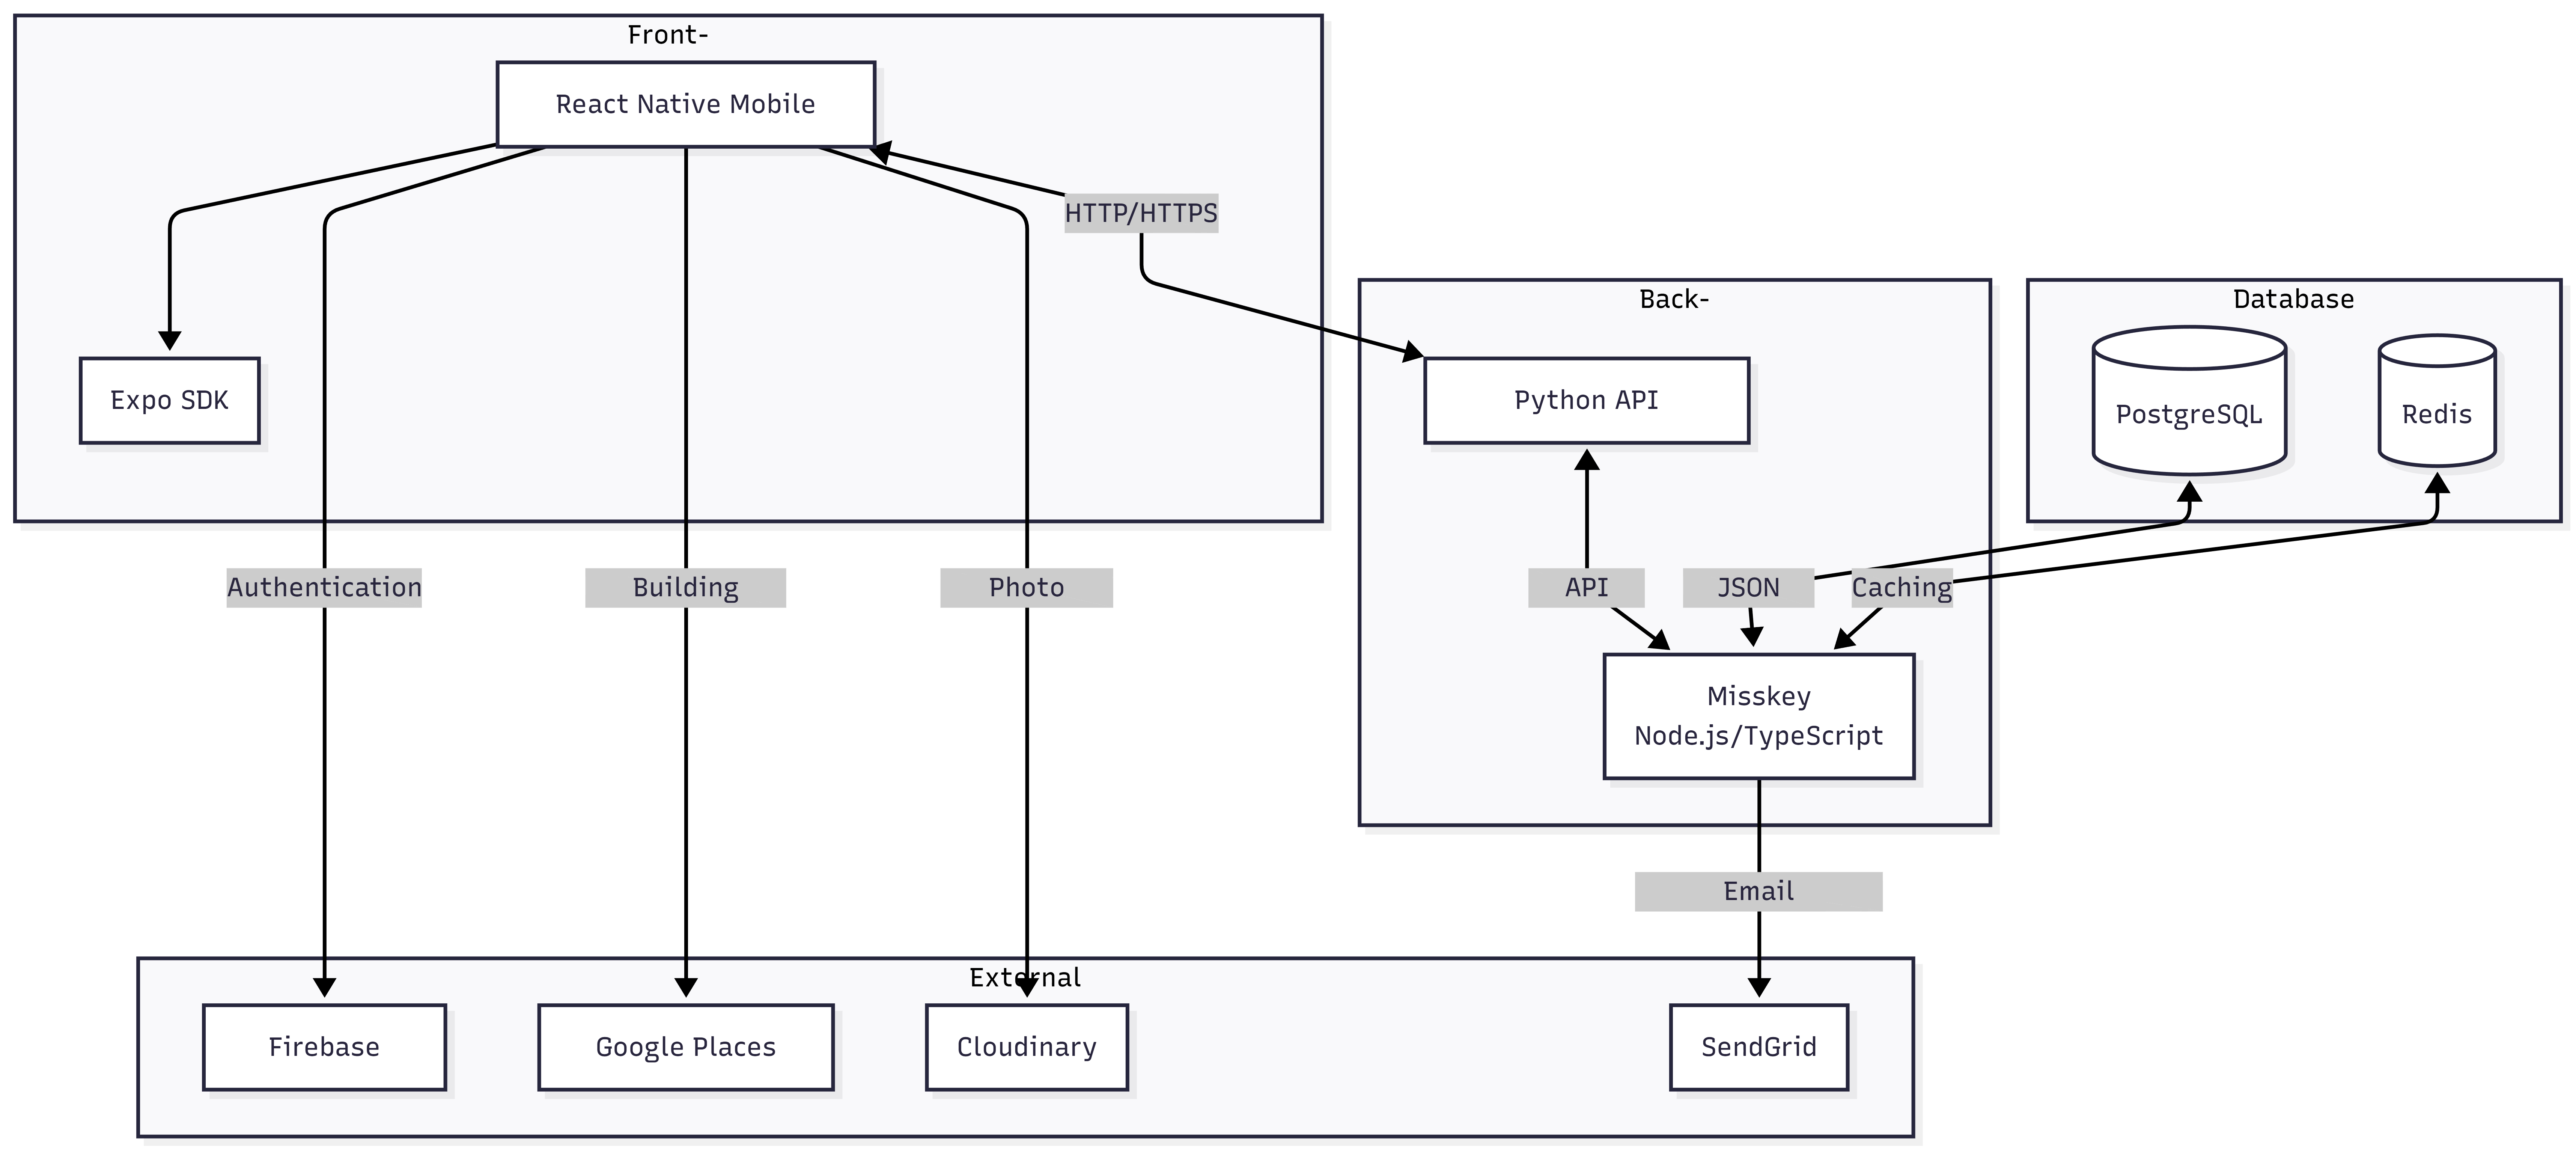
\includegraphics[width=\textwidth, keepaspectratio]{system/System_overview.png}
\caption{System Architecture Diagram}
\label{fig:system_architecture}
\end{figure}

Figure \ref{fig:system_architecture} above represents the architectural structure chosen for the development of the Infrastructure Degradation Management Platform. The system follows a three-tier architecture consisting of a database layer, back-end layer, and front-end layer.

The database layer utilizes PostgreSQL for persistent data storage of users, buildings, and reported issues, while Redis provides caching capabilities for improved performance. The back-end layer is built on Misskey, a Node.js and TypeScript-based social networking platform that provides fast, efficient infrastructure with built-in user management, post/timeline features, and database integration. To accommodate team members more familiar with Python, a Python API wrapper interfaces with the Misskey backend, allowing Python-based development while maintaining the core Misskey functionality.

The front-end layer consists of a React Native mobile application built with the Expo SDK, which provides camera and location APIs for photo capture and GPS coordinate retrieval. The mobile app communicates with the back-end through the Python API wrapper via HTTP/HTTPS requests.

The system integrates with several external services: Cloudinary for photo storage and processing, Google Places API for building identification based on GPS coordinates, Firebase Authentication for user account management, and SendGrid for email notifications to property associations. Currently, the notification system sends emails to associations when new issues are reported, though this can be extended to support additional notification methods in the future.

Storing information about users, buildings, and reported issues enables the system to maintain building records, track issue timelines, and manage notification history. User information enables the system to maintain user profiles and keep records of their reported issues.

Additionally, by following this architecture and structure, the system can be extended into additional features such as municipality dashboards, public record exports, and enhanced notification systems beyond email. However, this is out of the scope of this project and will be addressed in a future version.

\section{System Components}

\subsection{Decomposition Description}

\begin{figure}[H]
\centering
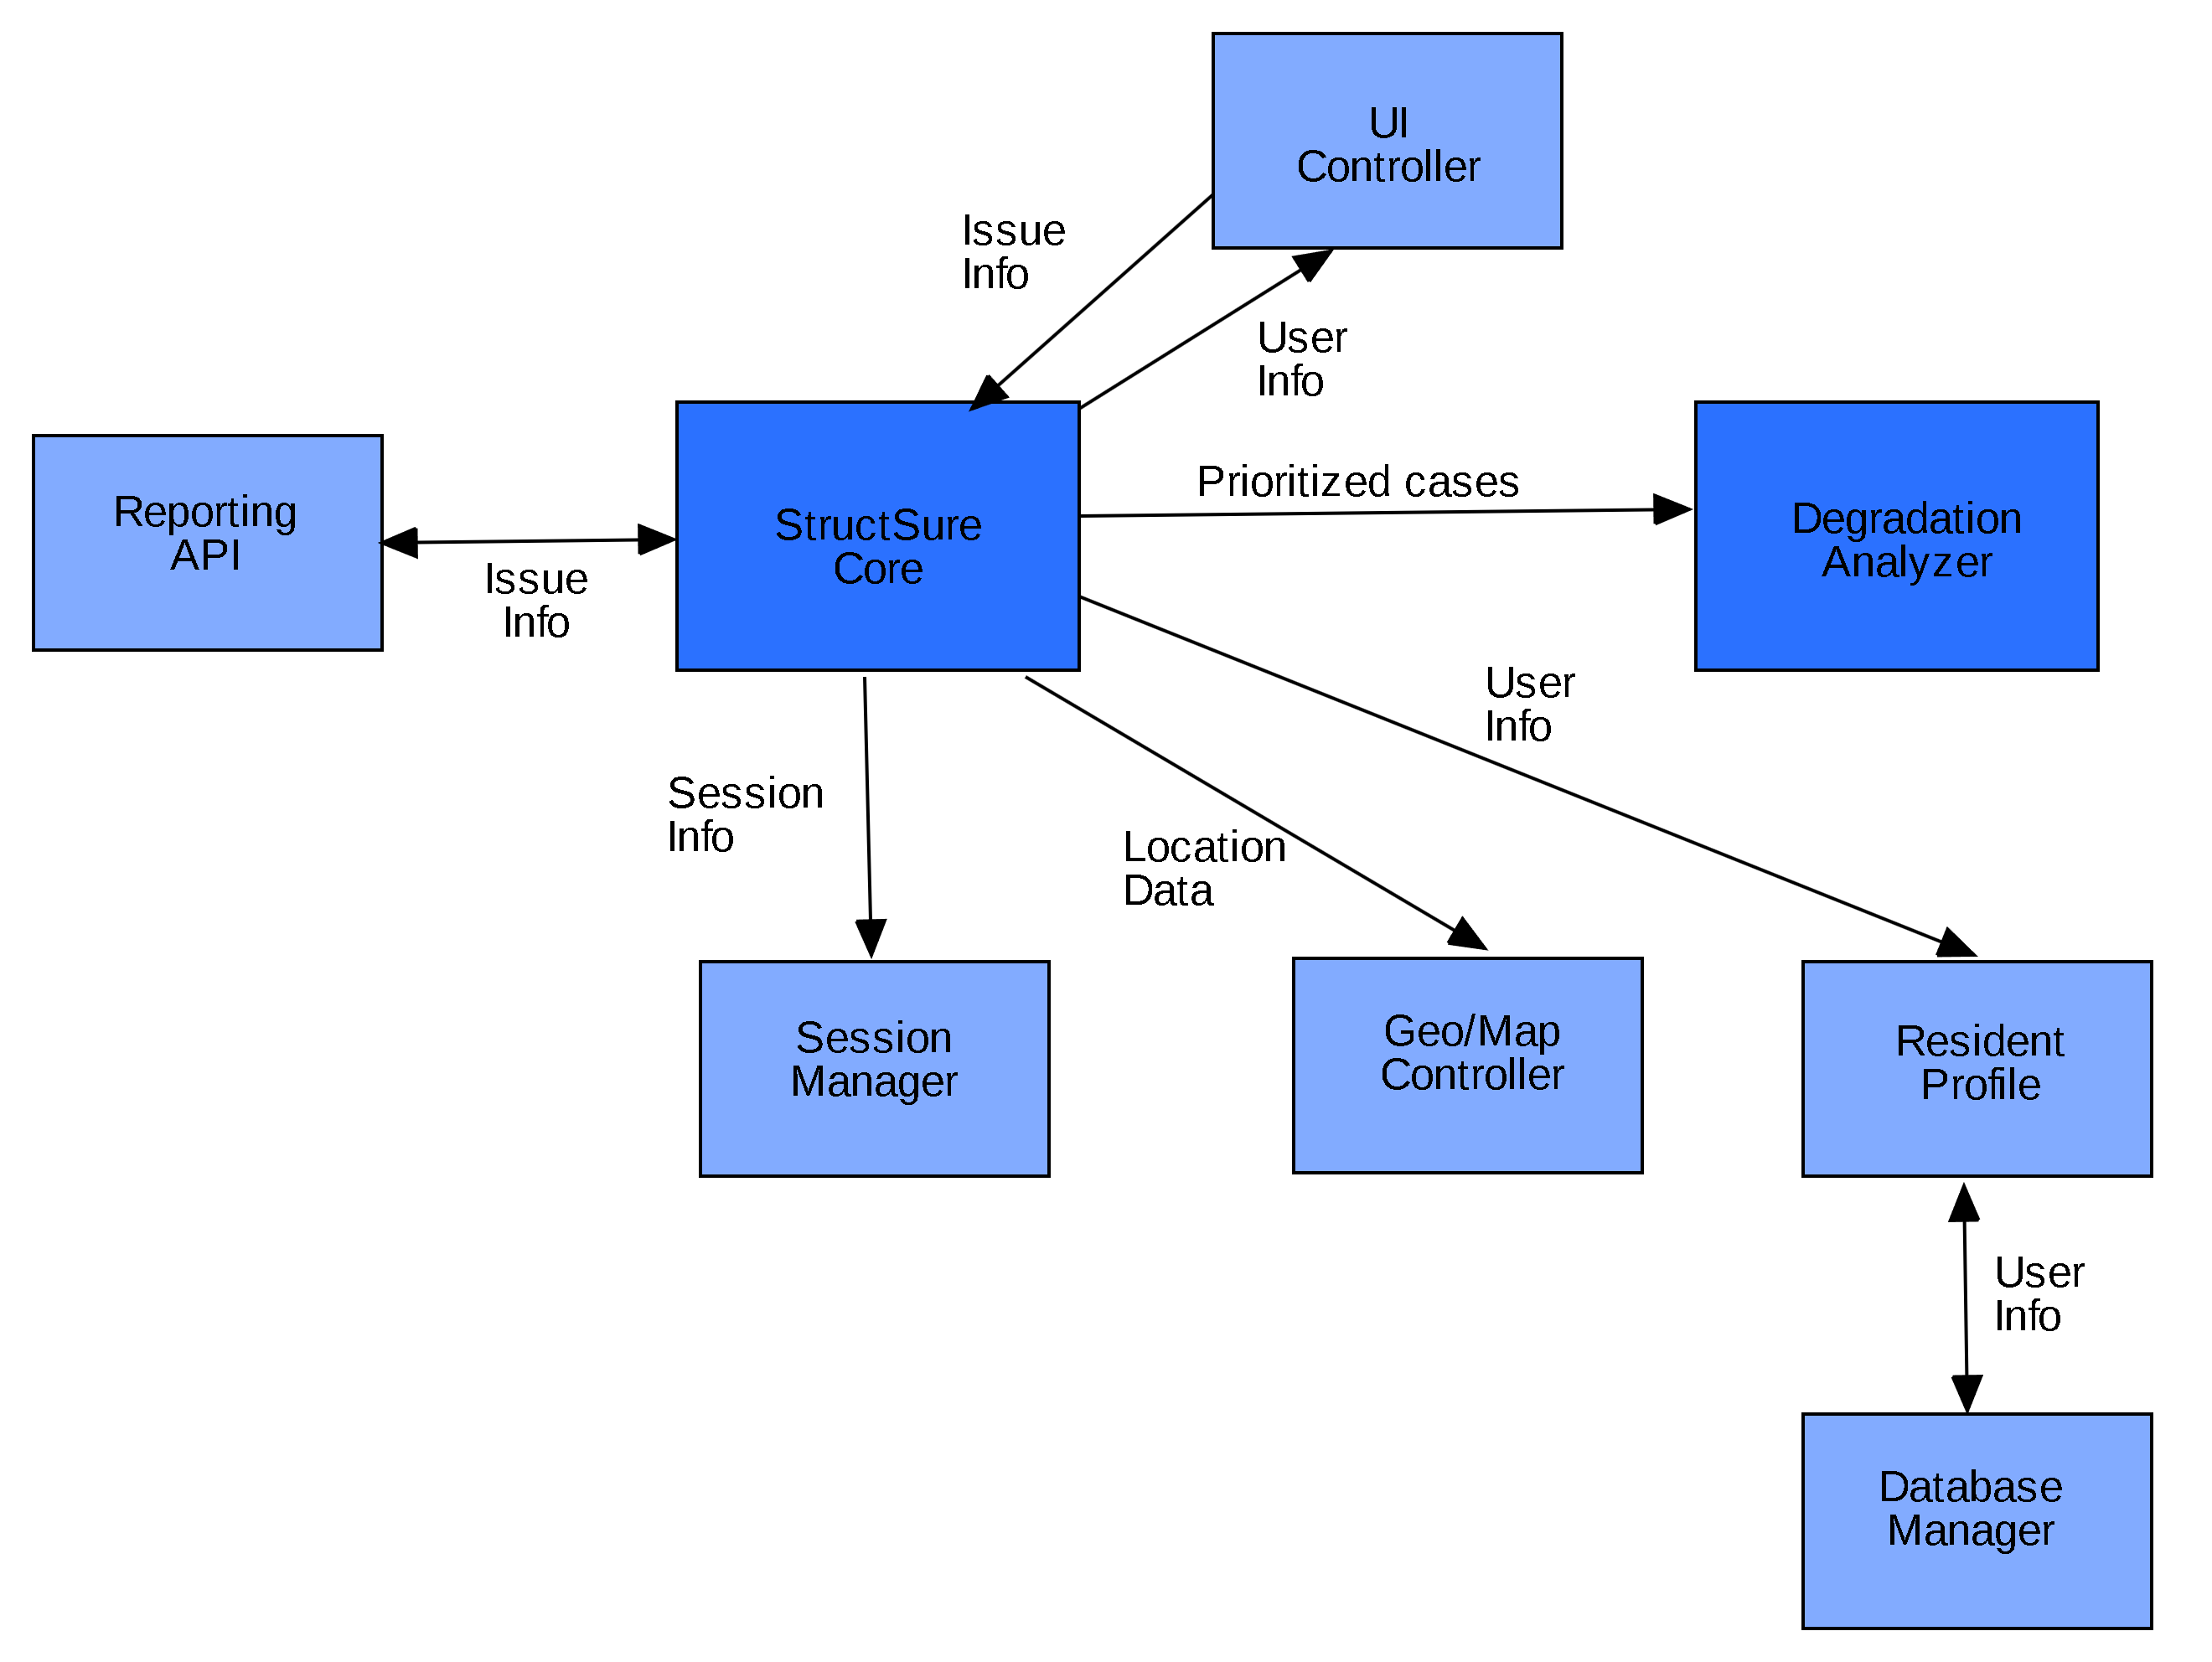
\includegraphics[width=\textwidth, keepaspectratio]{architecture/Decomposition.png}
\caption{System Decomposition Diagram}
\label{fig:decomposition}
\end{figure}

Figure \ref{fig:decomposition} above shows a top-down description of how the application is expected to work and how components will interact with one another. This logical component view complements the technology implementation view described in Section 2. The system consists of several key components:

The \textbf{UI Controller} is the main entry point for users, implemented as a React Native mobile application with the Expo SDK. It provides methods for capturing photos/videos, attaching location data, submitting reports, viewing status, and managing notifications.

The \textbf{StructSure Core} serves as the central orchestrator, implemented using the Misskey backend framework with a Python API wrapper. It coordinates interactions between all system components and manages the overall application flow.

The \textbf{Reporting API} handles report management and is implemented as part of the Misskey backend with Python API interfaces. It provides methods for creating reports, updating reports, adding evidence, listing reports, and exporting/sharing reports.

The \textbf{Session Manager} manages user authentication, implemented using Firebase Authentication. It provides methods for sign up, login, logout, and user validation.

The \textbf{Geo/Map Controller} handles geographical and map-related operations, integrating with the Google Places API. It provides methods to render maps, add markers, and show directions for building identification.

The \textbf{Resident Profile} manages resident-specific data including identity, address, association information, and notification preferences. This component utilizes the user management capabilities of Misskey.

The \textbf{Degradation Analyzer} performs analysis on reported issues to assess severity, detect duplicates, and prioritize cases. This component implements custom logic within the Misskey backend to analyze infrastructure degradation patterns.

The \textbf{Database Manager} handles all data persistence, implemented using PostgreSQL for persistent storage and Redis for caching. It provides methods to add/update users and reports, retrieve reports, and delete reports.

\subsection{Dependency Description}

\begin{figure}[H]
\centering
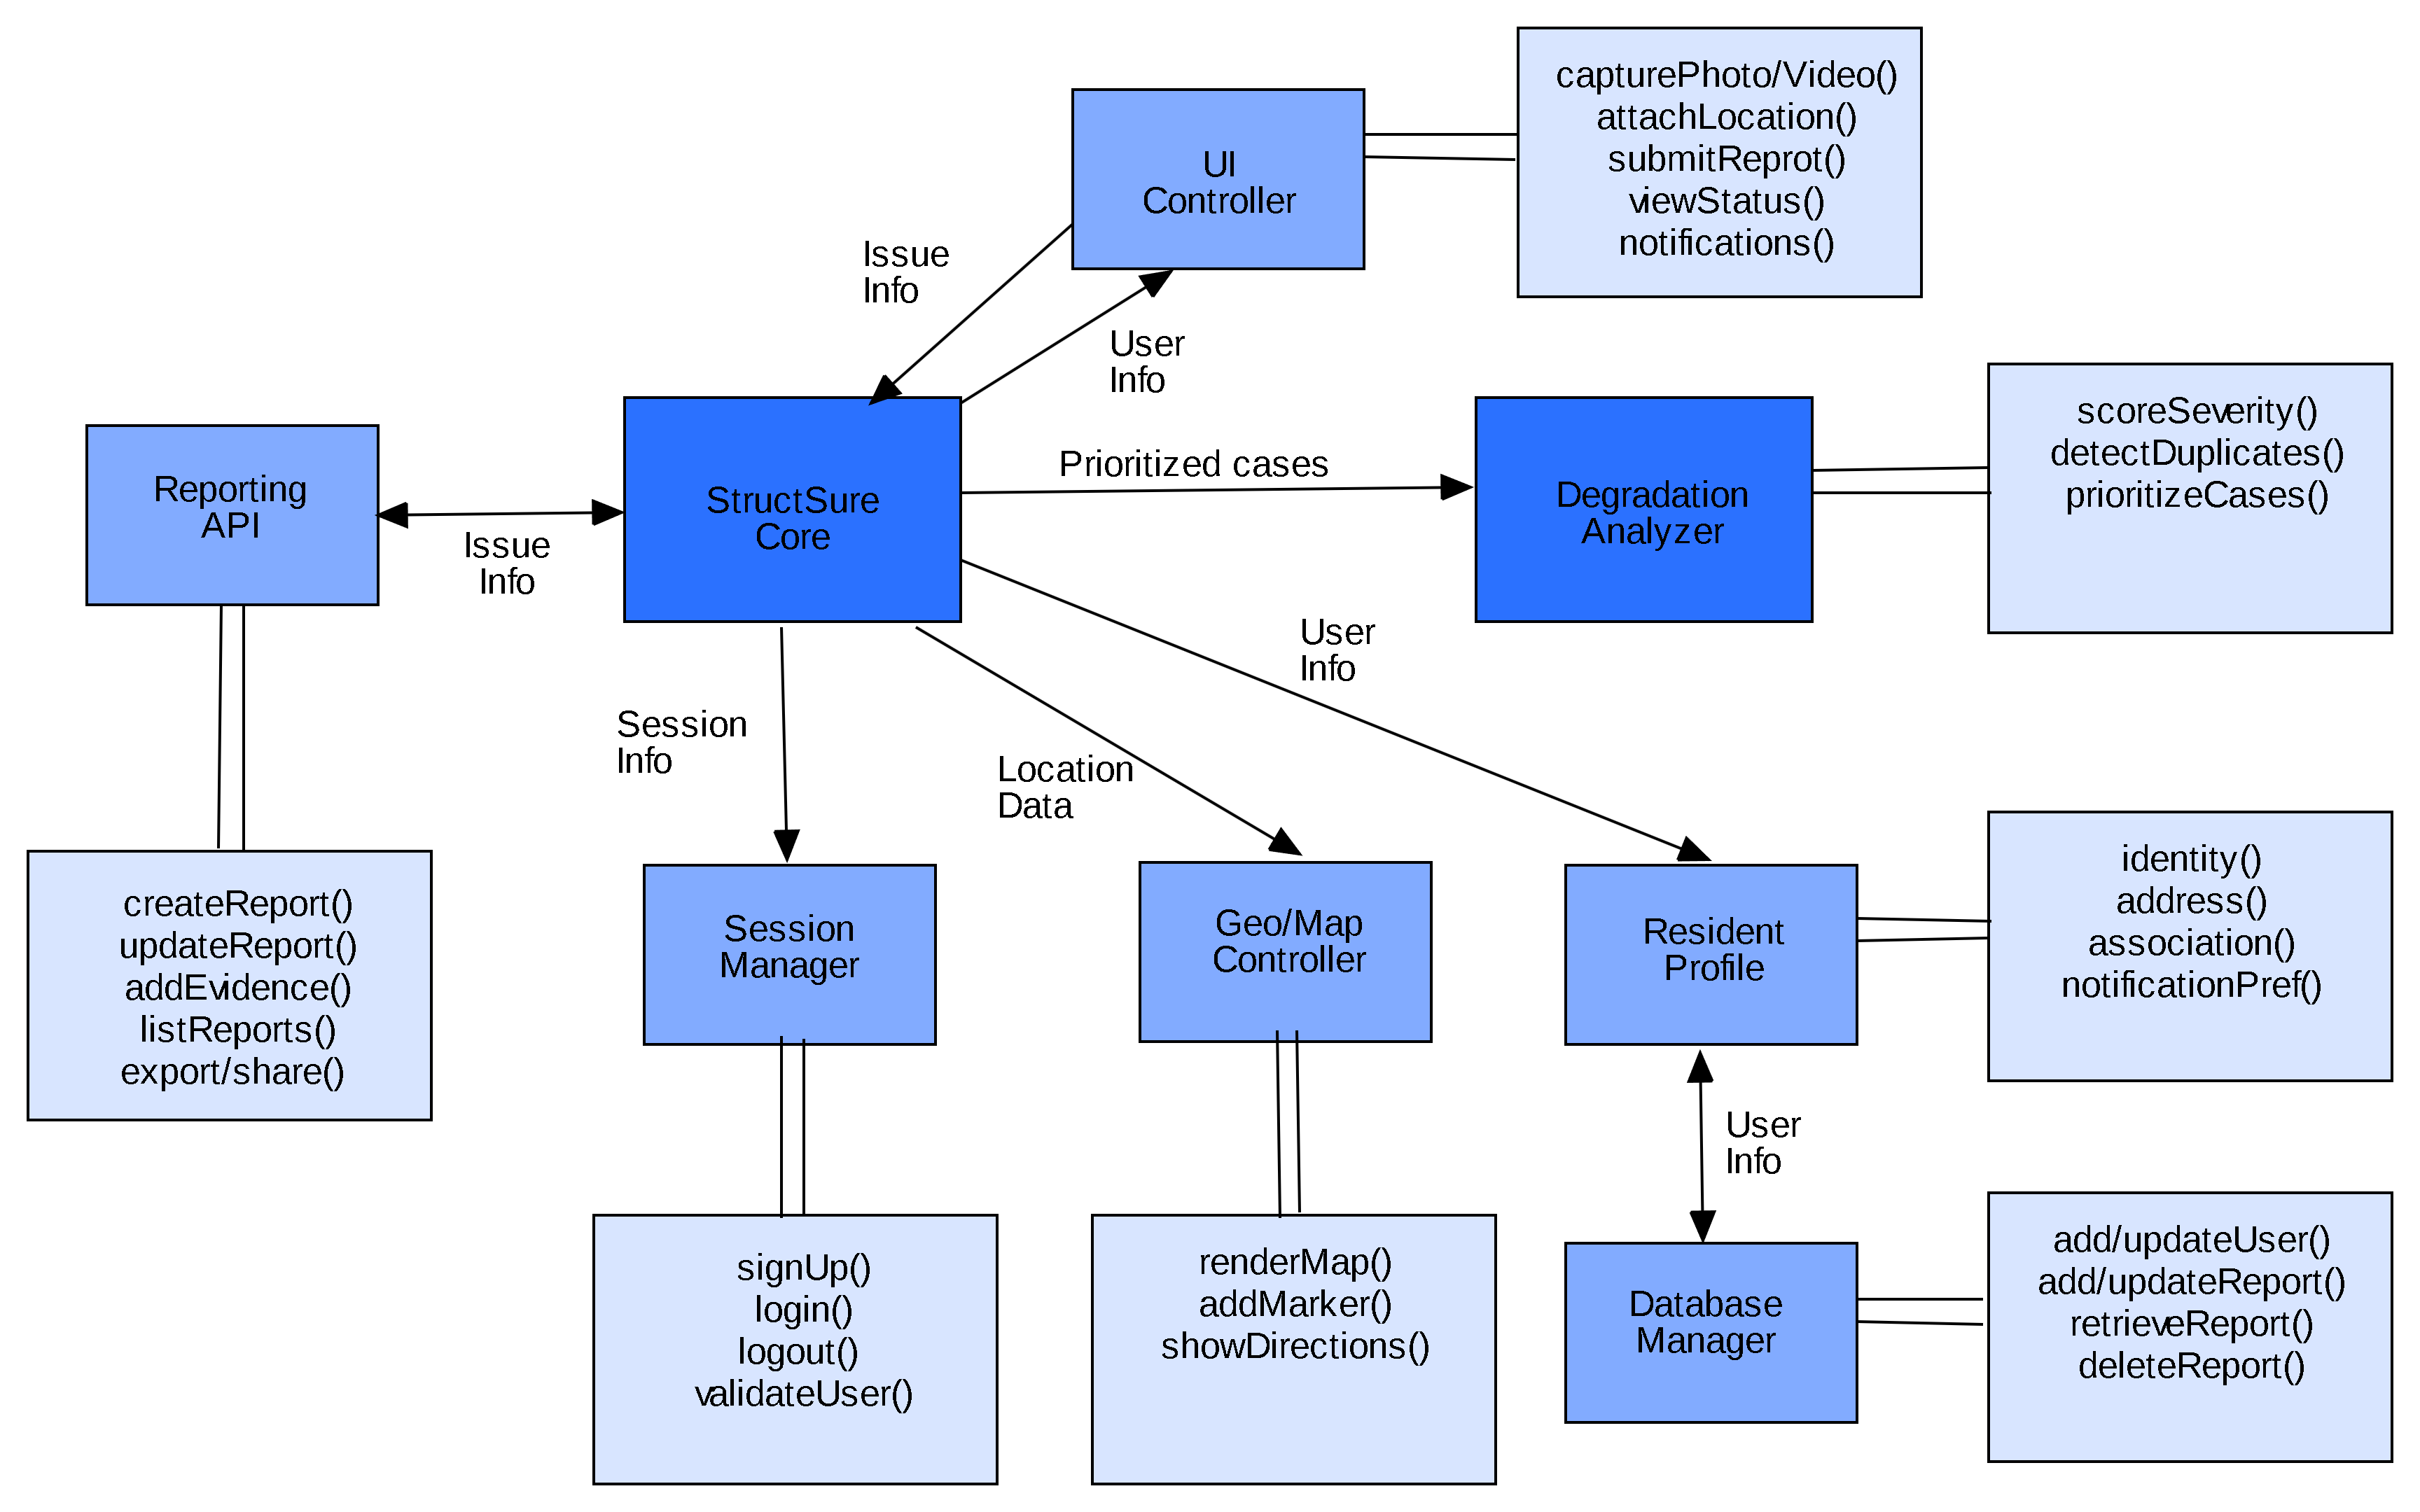
\includegraphics[width=\textwidth, keepaspectratio]{architecture/Dependency.png}
\caption{System Dependency Diagram}
\label{fig:dependency}
\end{figure}

Figure \ref{fig:dependency} above represents the component diagram of the system and how each module is dependent on another for its functionality. This diagram illustrates the logical flow and dependencies between components, which are implemented using the technology stack described in Section 2.

The UI Controller, implemented as a React Native mobile application, initiates user interactions and communicates with the StructSure Core, which serves as the central processing unit implemented using Misskey with a Python API wrapper. The StructSure Core orchestrates interactions with specialized components: the Reporting API for managing issue reports, the Session Manager (Firebase Authentication) for user authentication, the Geo/Map Controller (Google Places API integration) for location and mapping services, and the Degradation Analyzer for analyzing reported infrastructure issues.

The Session Manager handles user authentication through Firebase Authentication and communicates directly with the Database Manager (PostgreSQL) to store and retrieve user session data. The Geo/Map Controller processes location information through the Google Places API and stores geographical data in the Database Manager. The Degradation Analyzer processes reported issues and interacts with the Resident Profile component, which manages resident information using Misskey's user management features and also stores data in the Database Manager.

The Reporting API, implemented through the Misskey backend and Python API wrapper, creates report posts that are stored in the Database Manager. When photos are captured through the UI Controller, they are uploaded to Cloudinary for storage and processing. When new issue reports are created, the system retrieves association contact information from the database and sends email notifications via SendGrid.

The Database Manager serves as the central data persistence layer, implemented using PostgreSQL for persistent storage and Redis for caching. It receives data from the Session Manager, Geo/Map Controller, and Resident Profile components. All user data, building records, reported issues, and associated information are stored in the database to maintain system state and enable retrieval of historical data.

For detailed dependency information, see Dependency\_Description.md.

\subsection{Interface Description}

\subsubsection{UI Controller Component}

\begin{figure}[H]
\centering
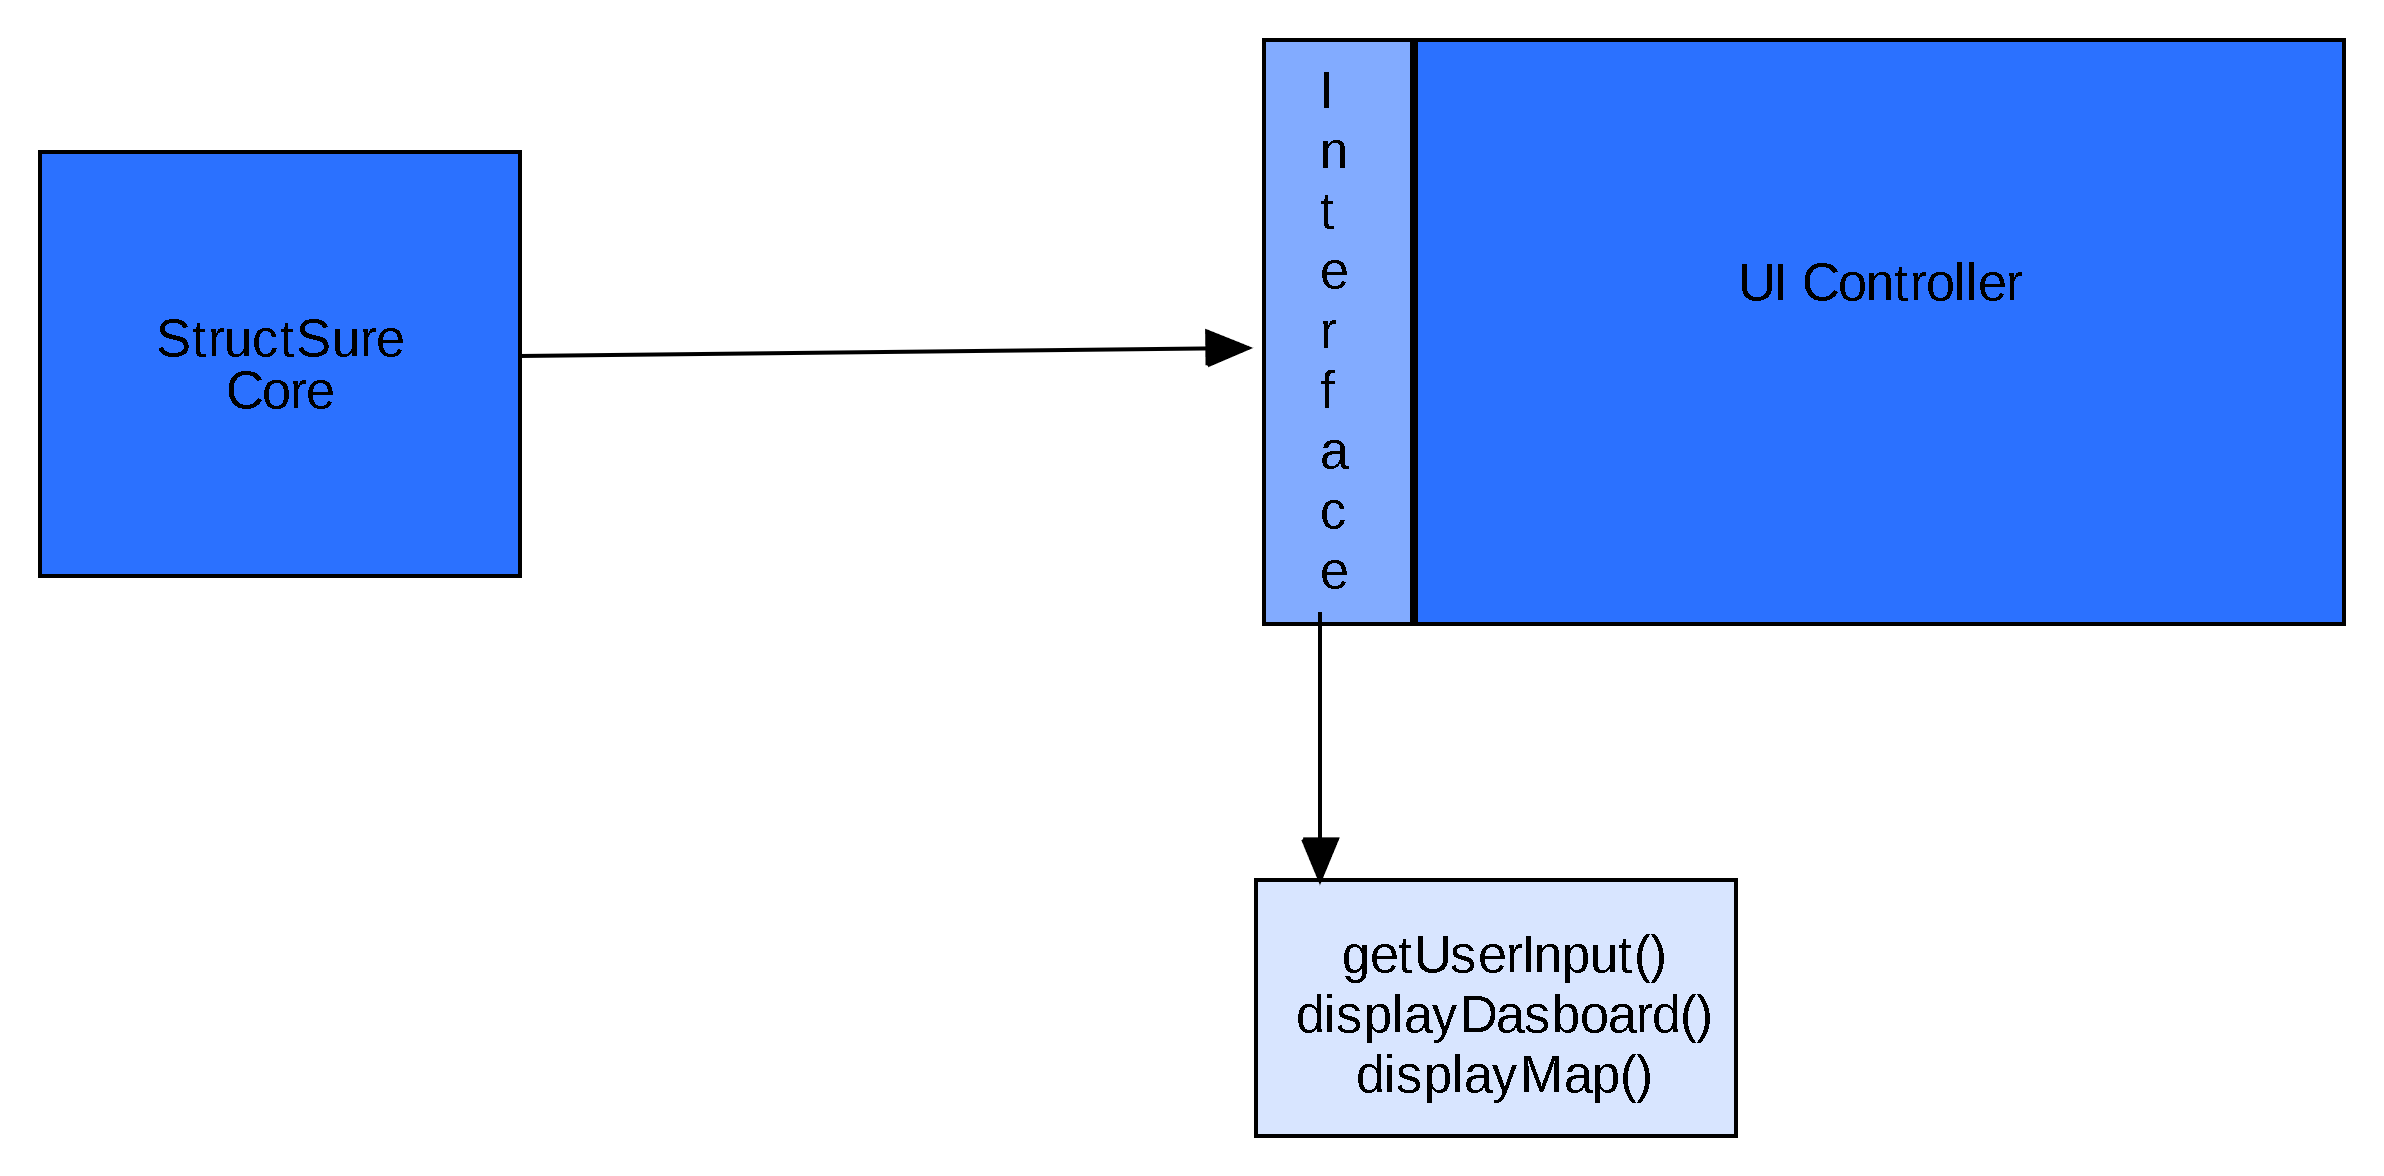
\includegraphics[height=0.2\textheight, keepaspectratio]{architecture/UI_Controller.png}
\caption{UI Controller Interface}
\label{fig:ui_controller}
\end{figure}

Figure \ref{fig:ui_controller} above shows the UI Controller interface. The UI Controller communicates with the StructSure Core via HTTP/HTTPS requests through the Python API wrapper, routing user actions, photo data, location information, and report details.

\subsubsection{Session Manager and User Authentication}

\begin{figure}[H]
\centering
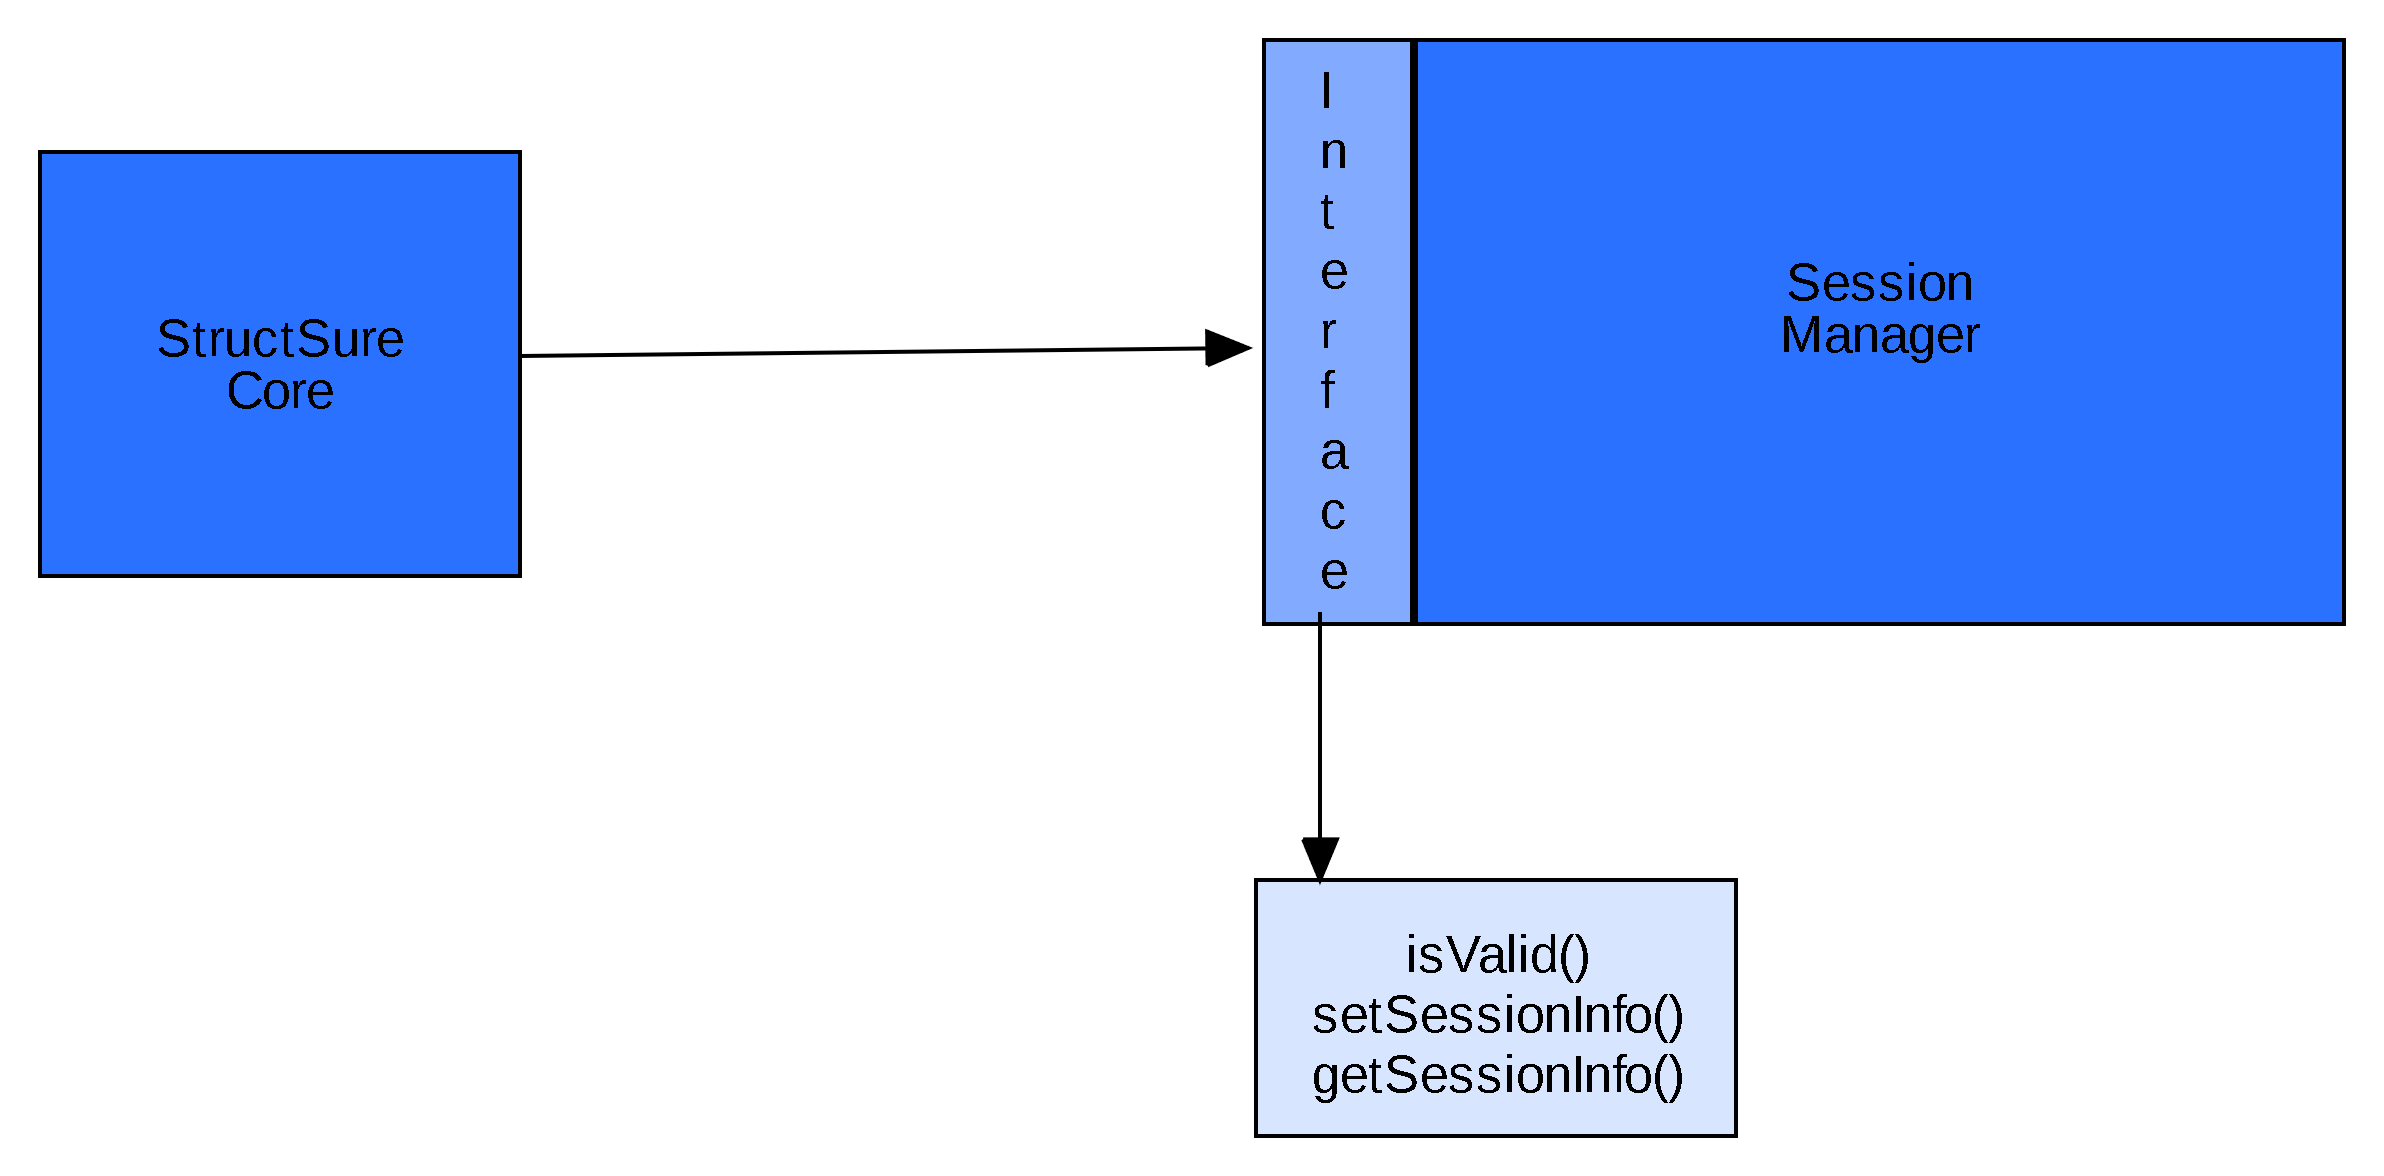
\includegraphics[height=0.2\textheight, keepaspectratio]{architecture/Session_Manager.png}
\hfill
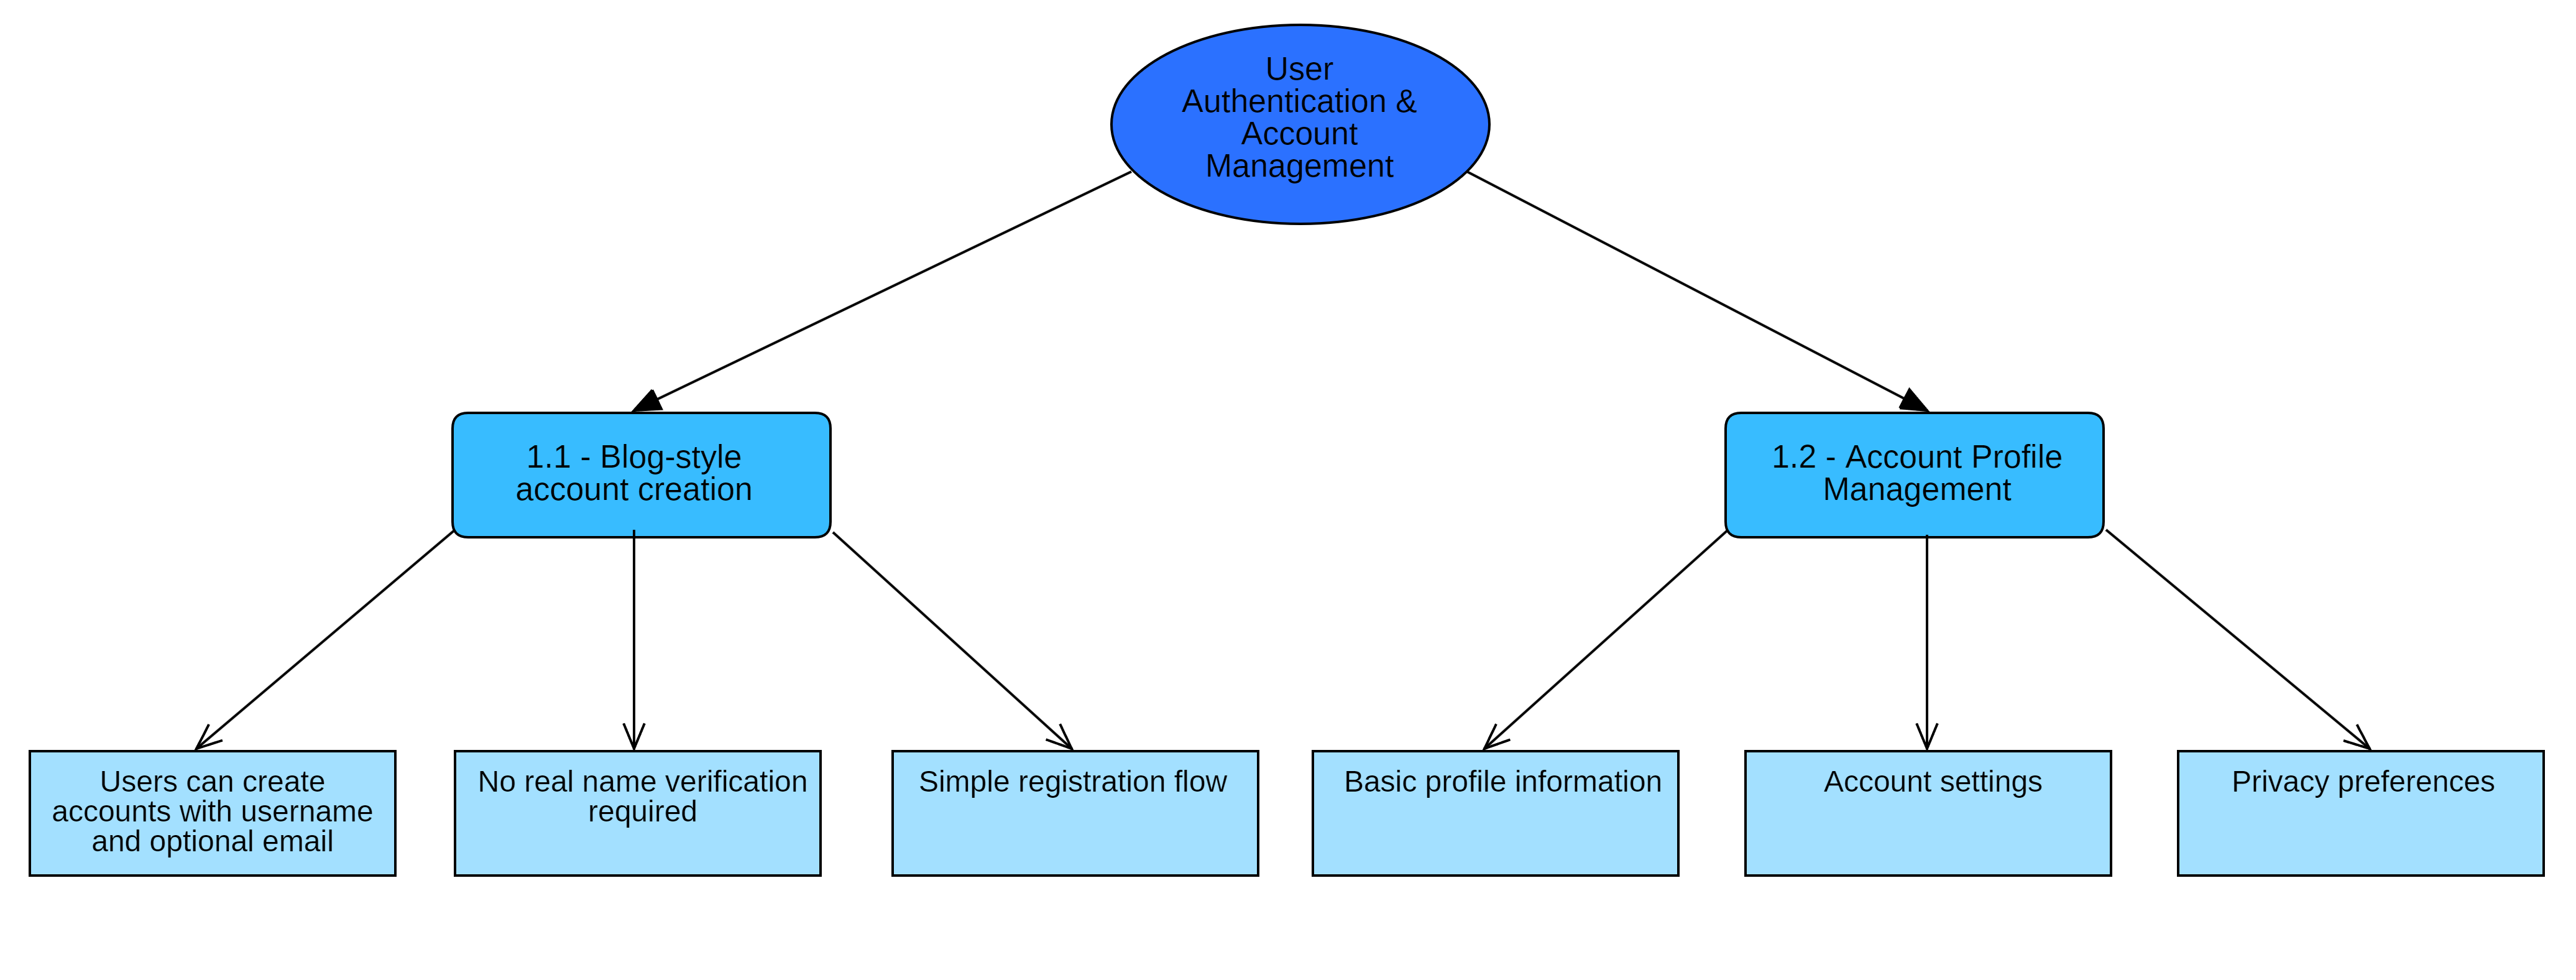
\includegraphics[height=0.2\textheight, keepaspectratio]{architecture/user_auth.png}
\caption{Session Manager and User Authentication Interfaces}
\label{fig:session_manager}
\end{figure}

Figure \ref{fig:session_manager} above shows the Session Manager authentication interface. The StructSure Core requests authentication status from the Session Manager before allowing system access. Unauthenticated users are redirected to the login screen, and the Session Manager validates credentials throughout the session.

\subsubsection{Photo Capture Authentication}

\begin{figure}[H]
\centering
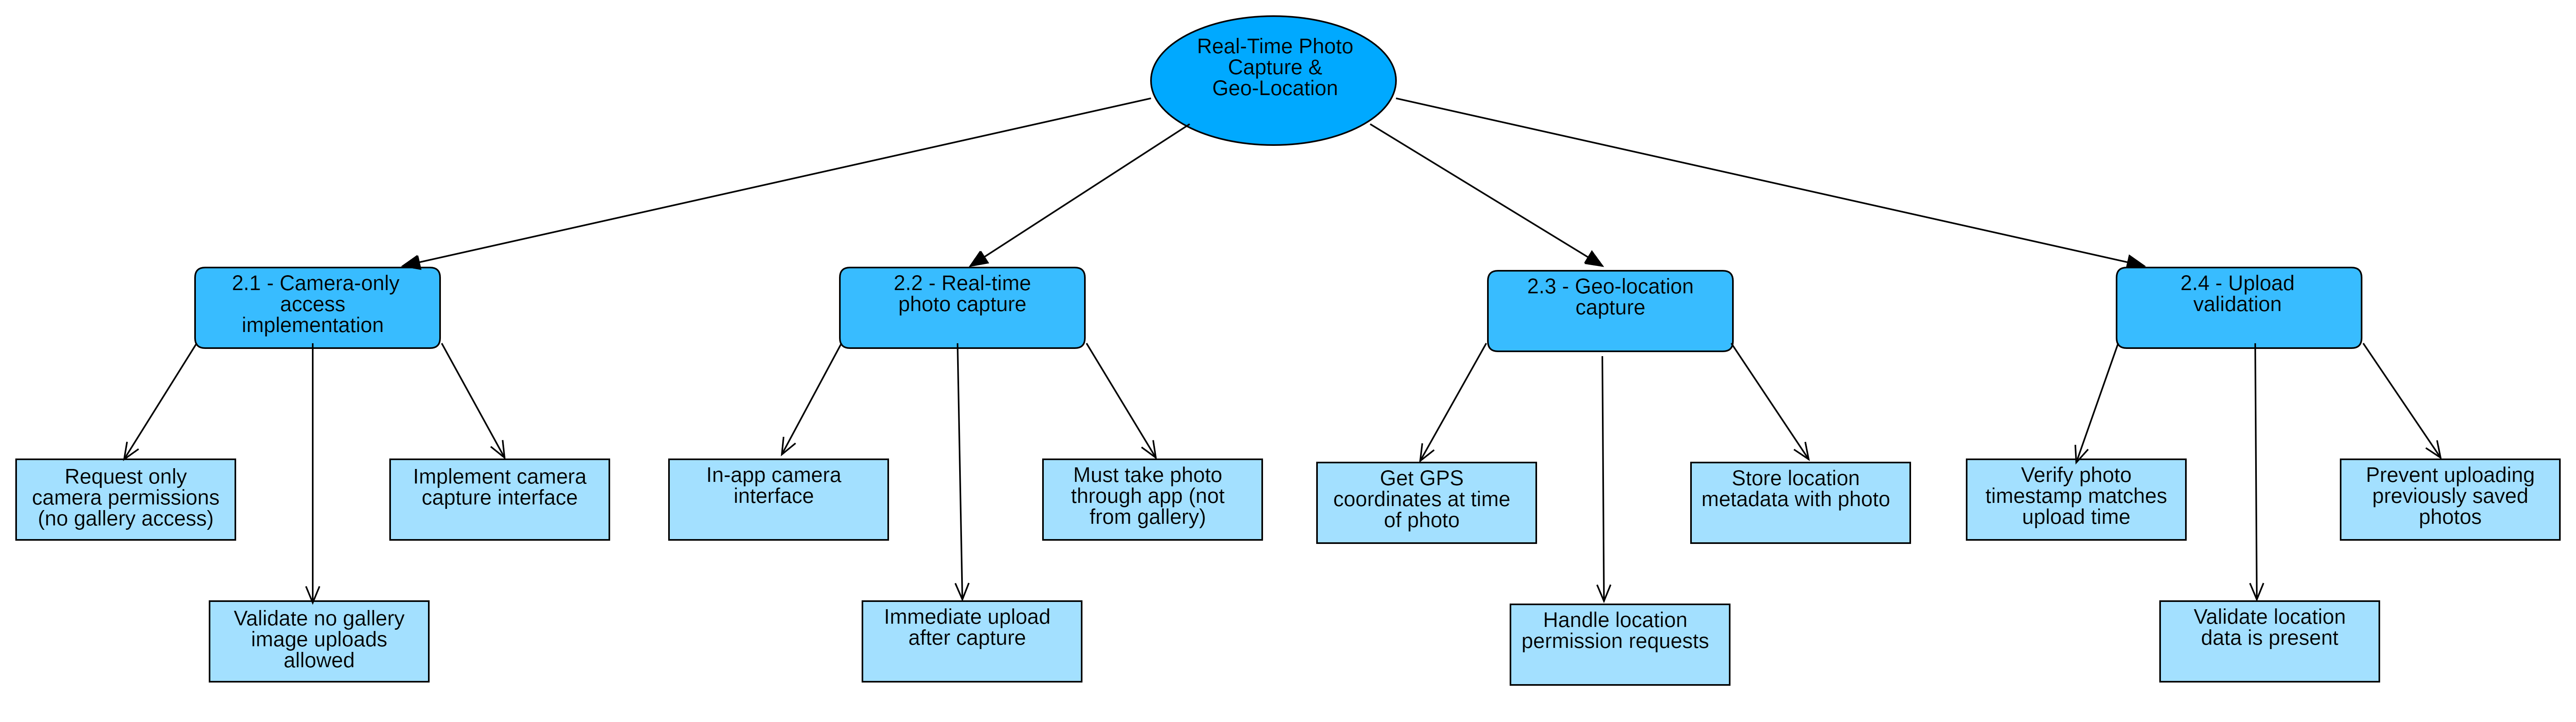
\includegraphics[height=0.2\textheight, keepaspectratio]{architecture/photo_auth.png}
\caption{Photo Capture Authentication Interface}
\label{fig:photo_auth}
\end{figure}

Figure \ref{fig:photo_auth} above shows the Photo Capture Authentication interface. This interface handles authentication requirements specific to photo capture functionality, ensuring users are properly authenticated before capturing and uploading photos of infrastructure issues.

\subsubsection{Building Identification and Tagging}

\begin{figure}[H]
\centering
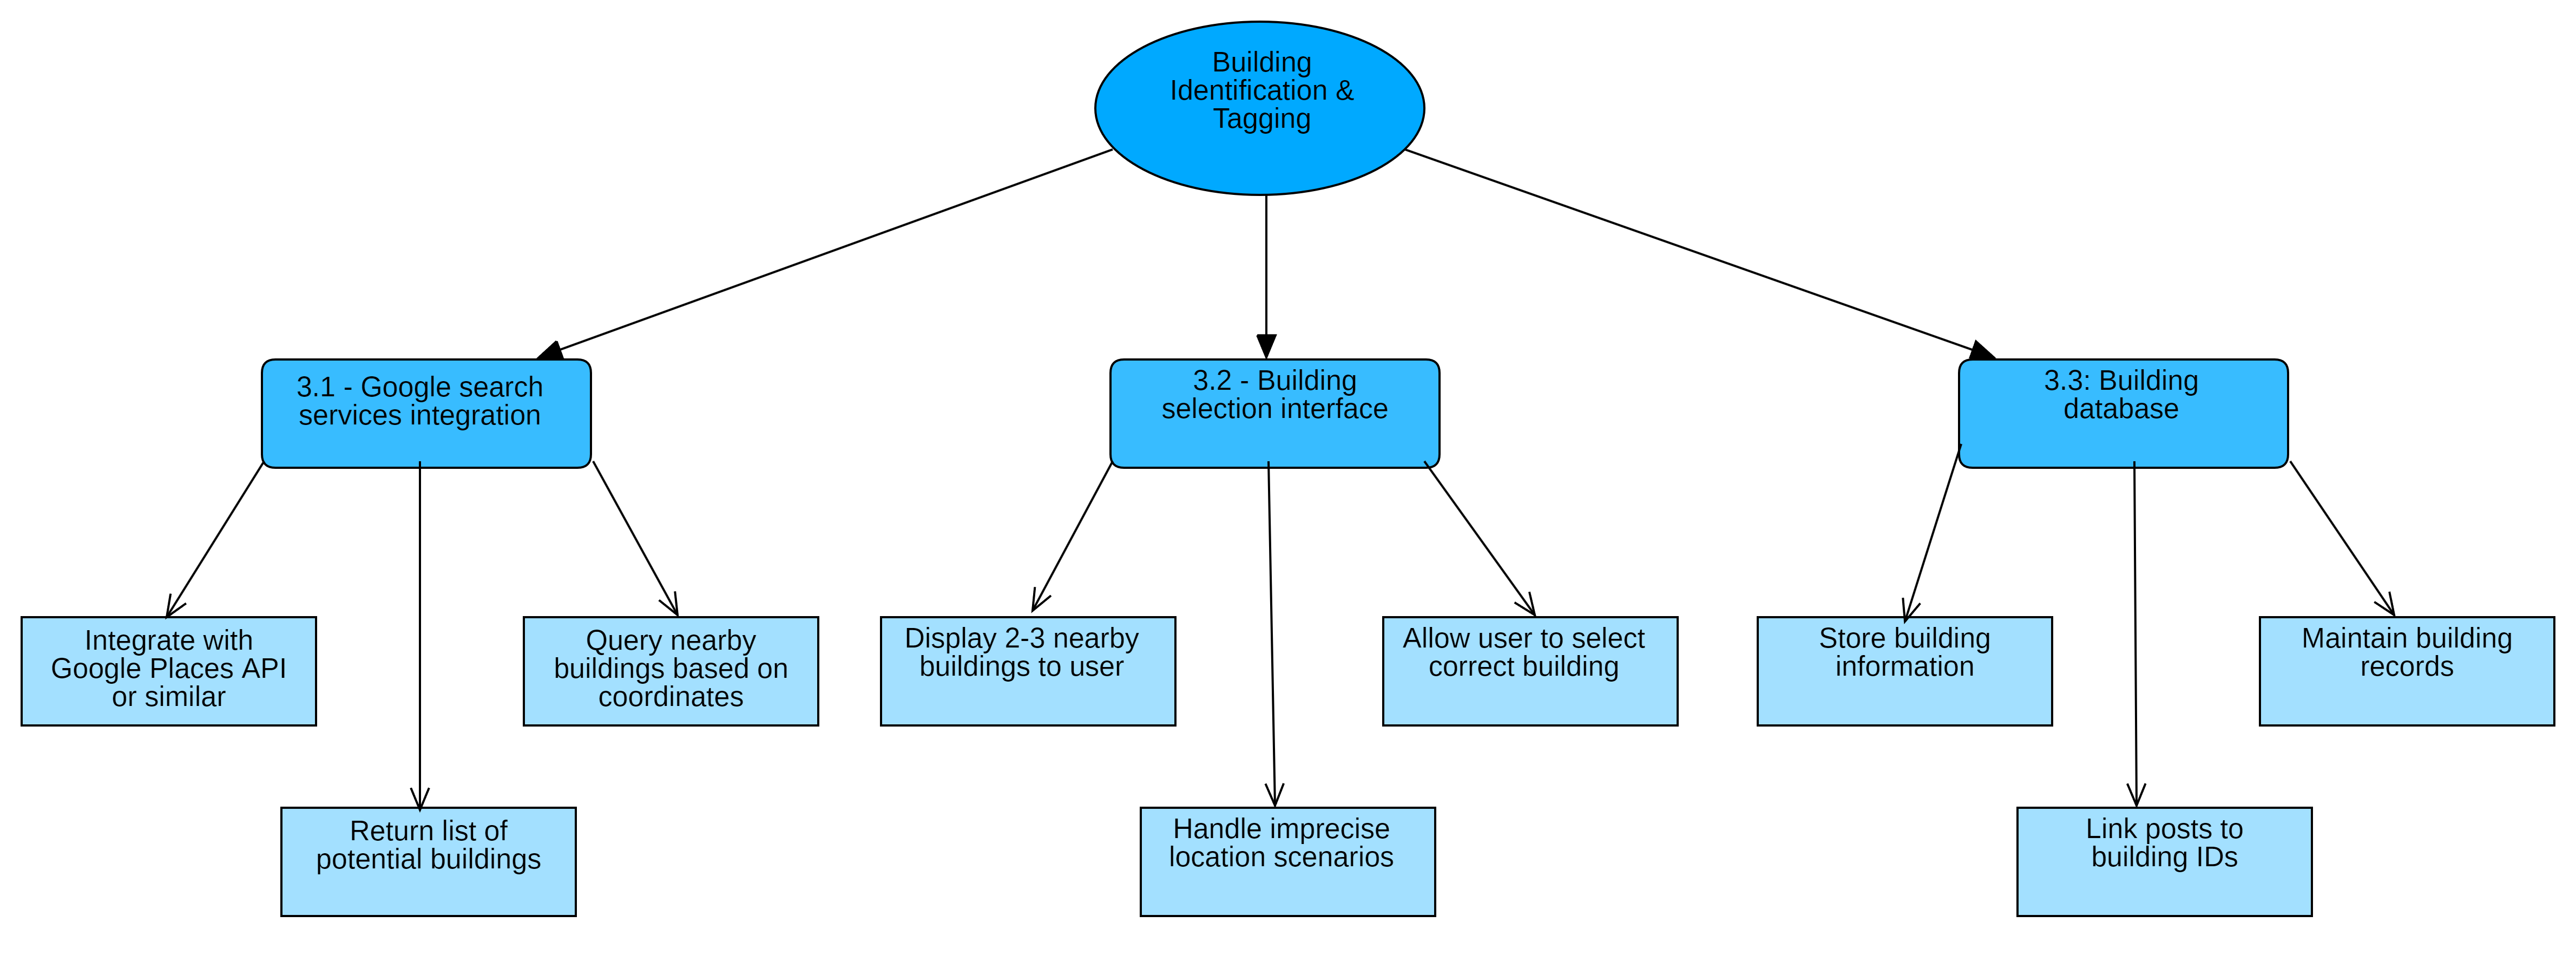
\includegraphics[height=0.2\textheight, keepaspectratio]{architecture/Building_identification_tagging.png}
\caption{Building Identification Interface}
\label{fig:building_id}
\end{figure}

Figure \ref{fig:building_id} above shows the Building Identification interface. When photos include location data, the system queries nearby buildings and presents 2-3 options for user selection. Selected buildings are stored and associated with reported issues.

\subsubsection{Issue Management}

\begin{figure}[H]
\centering
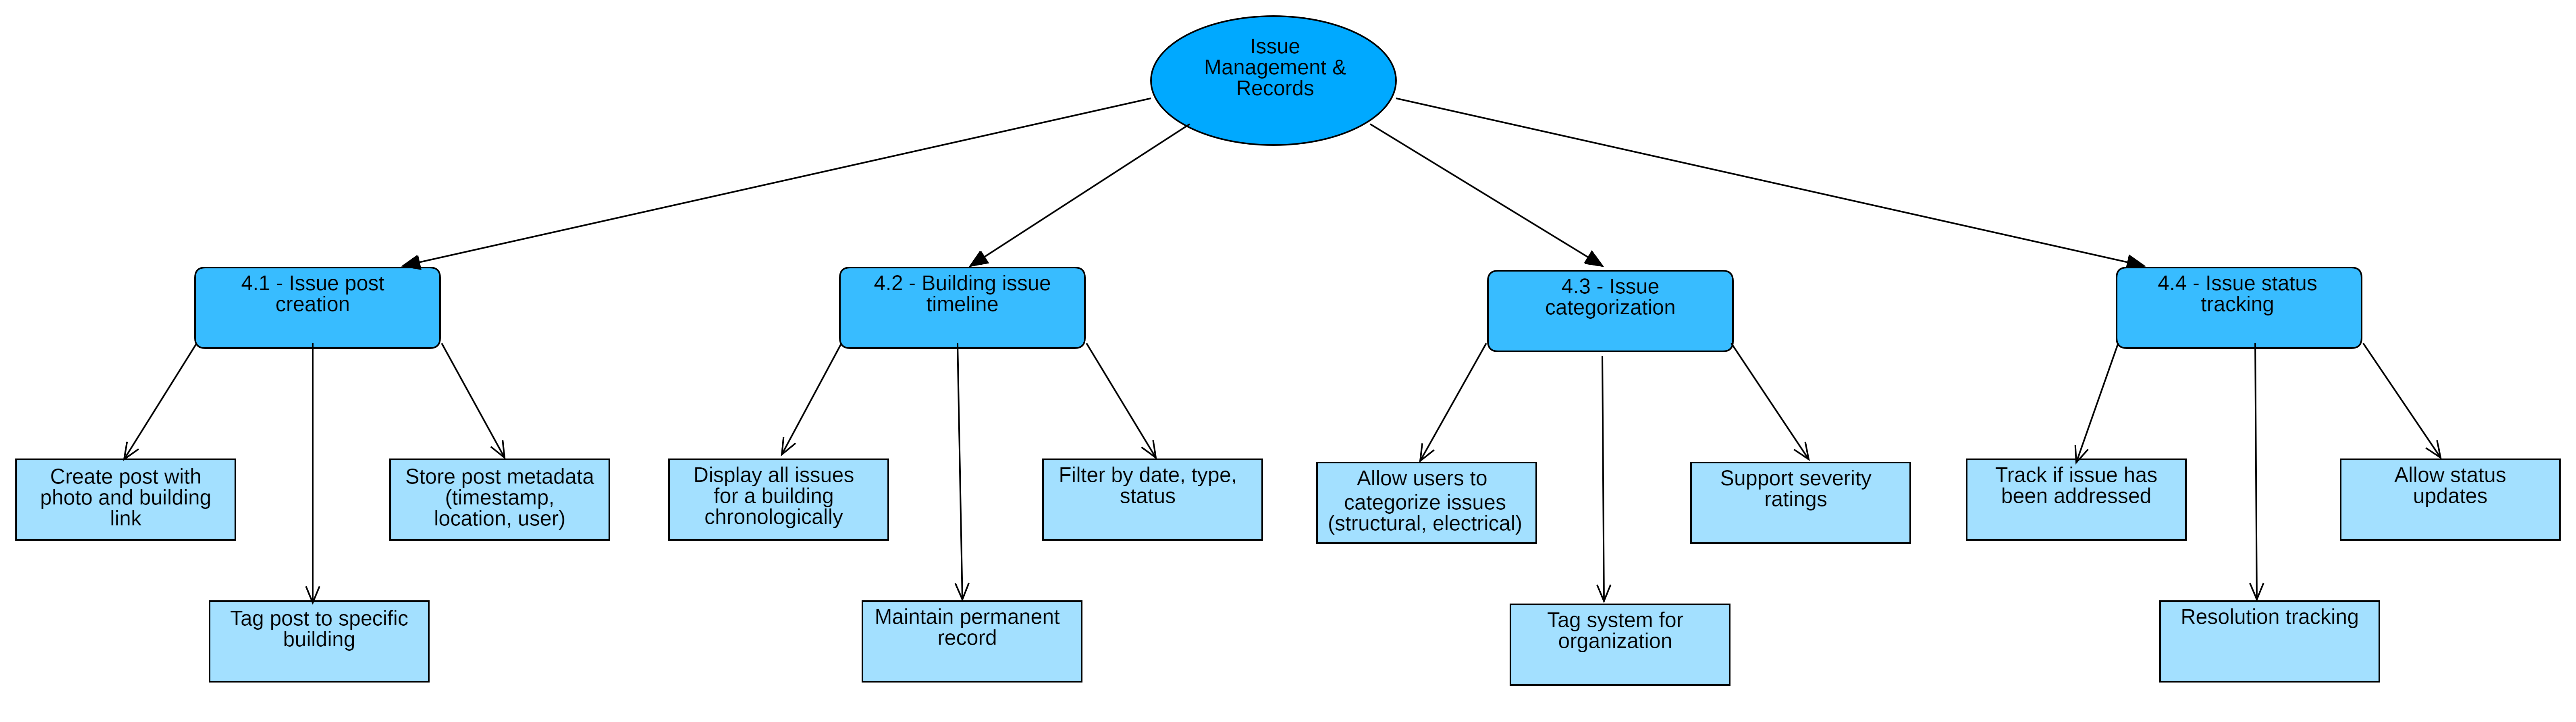
\includegraphics[height=0.2\textheight, keepaspectratio]{architecture/Issue_Management.png}
\caption{Issue Management Interface}
\label{fig:issue_management}
\end{figure}

Figure \ref{fig:issue_management} above shows the Issue Management interface. Reports include photo URLs, building associations, GPS coordinates, timestamps, and user information. Reports can be categorized, assigned severity ratings, and tracked for status updates.

\subsubsection{Resident Profile}

\begin{figure}[H]
\centering
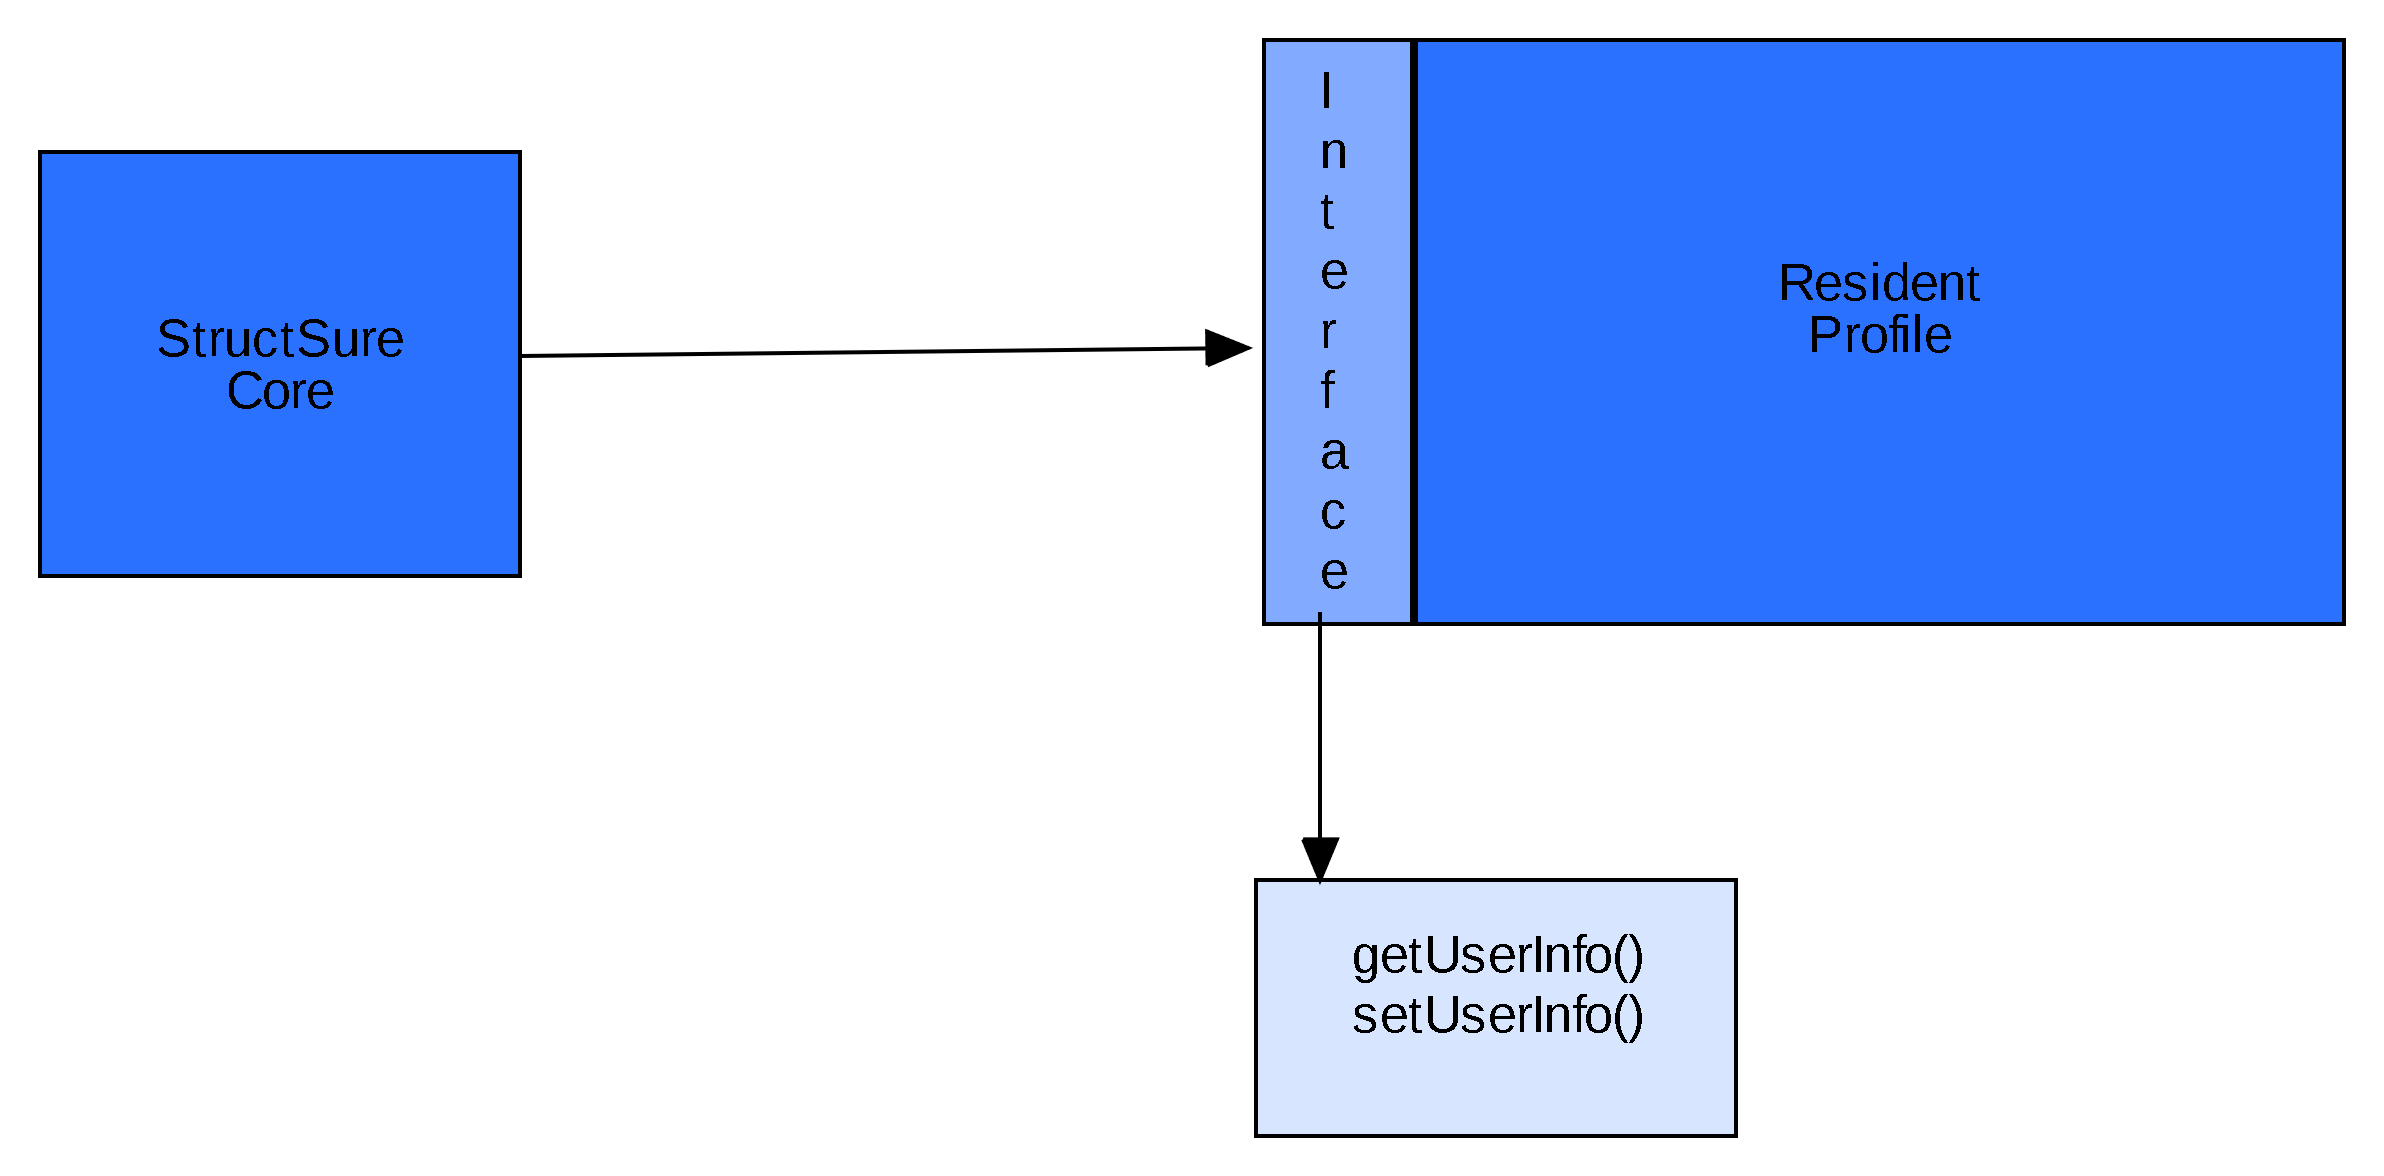
\includegraphics[height=0.2\textheight, keepaspectratio]{architecture/Resident_Profile.png}
\caption{Resident Profile Interface}
\label{fig:resident_profile}
\end{figure}

Figure \ref{fig:resident_profile} above shows the Resident Profile interface for managing resident identity, address, association information, and notification preferences. Profiles are linked to reported issues.

\subsubsection{Degradation Analyzer}

\begin{figure}[H]
\centering
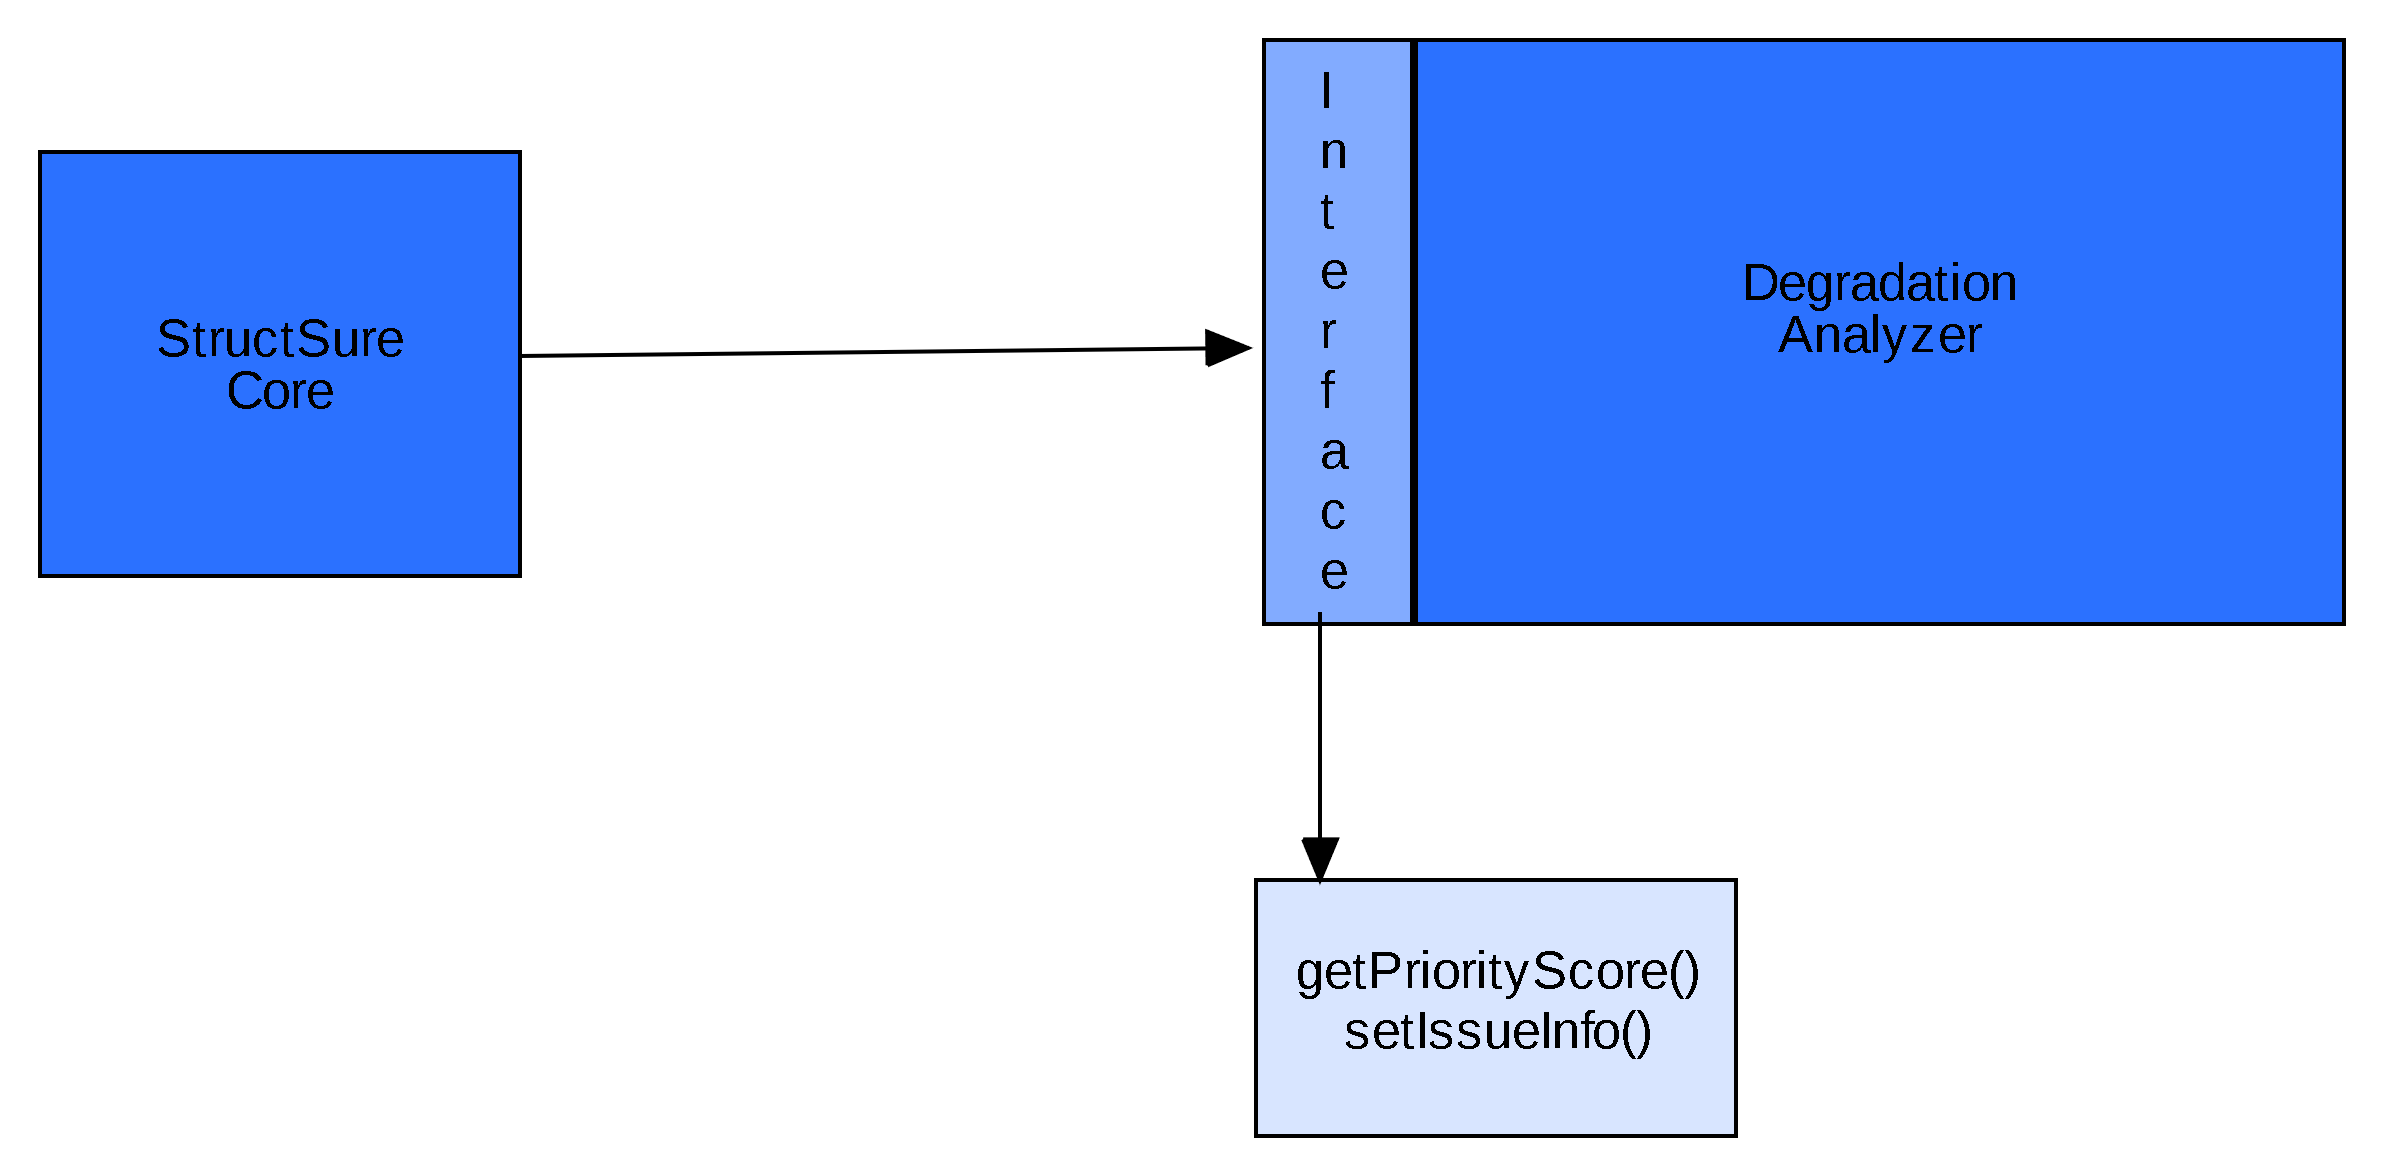
\includegraphics[height=0.2\textheight, keepaspectratio]{architecture/Dergradation_Analyzer.png}
\caption{Degradation Analyzer Interface}
\label{fig:degradation_analyzer}
\end{figure}

Figure \ref{fig:degradation_analyzer} above shows the Degradation Analyzer interface for assessing issue severity, detecting duplicates, and prioritizing cases. The analyzer interacts with the Resident Profile component to update relevant data.

\subsubsection{Association Management}

\begin{figure}[H]
\centering
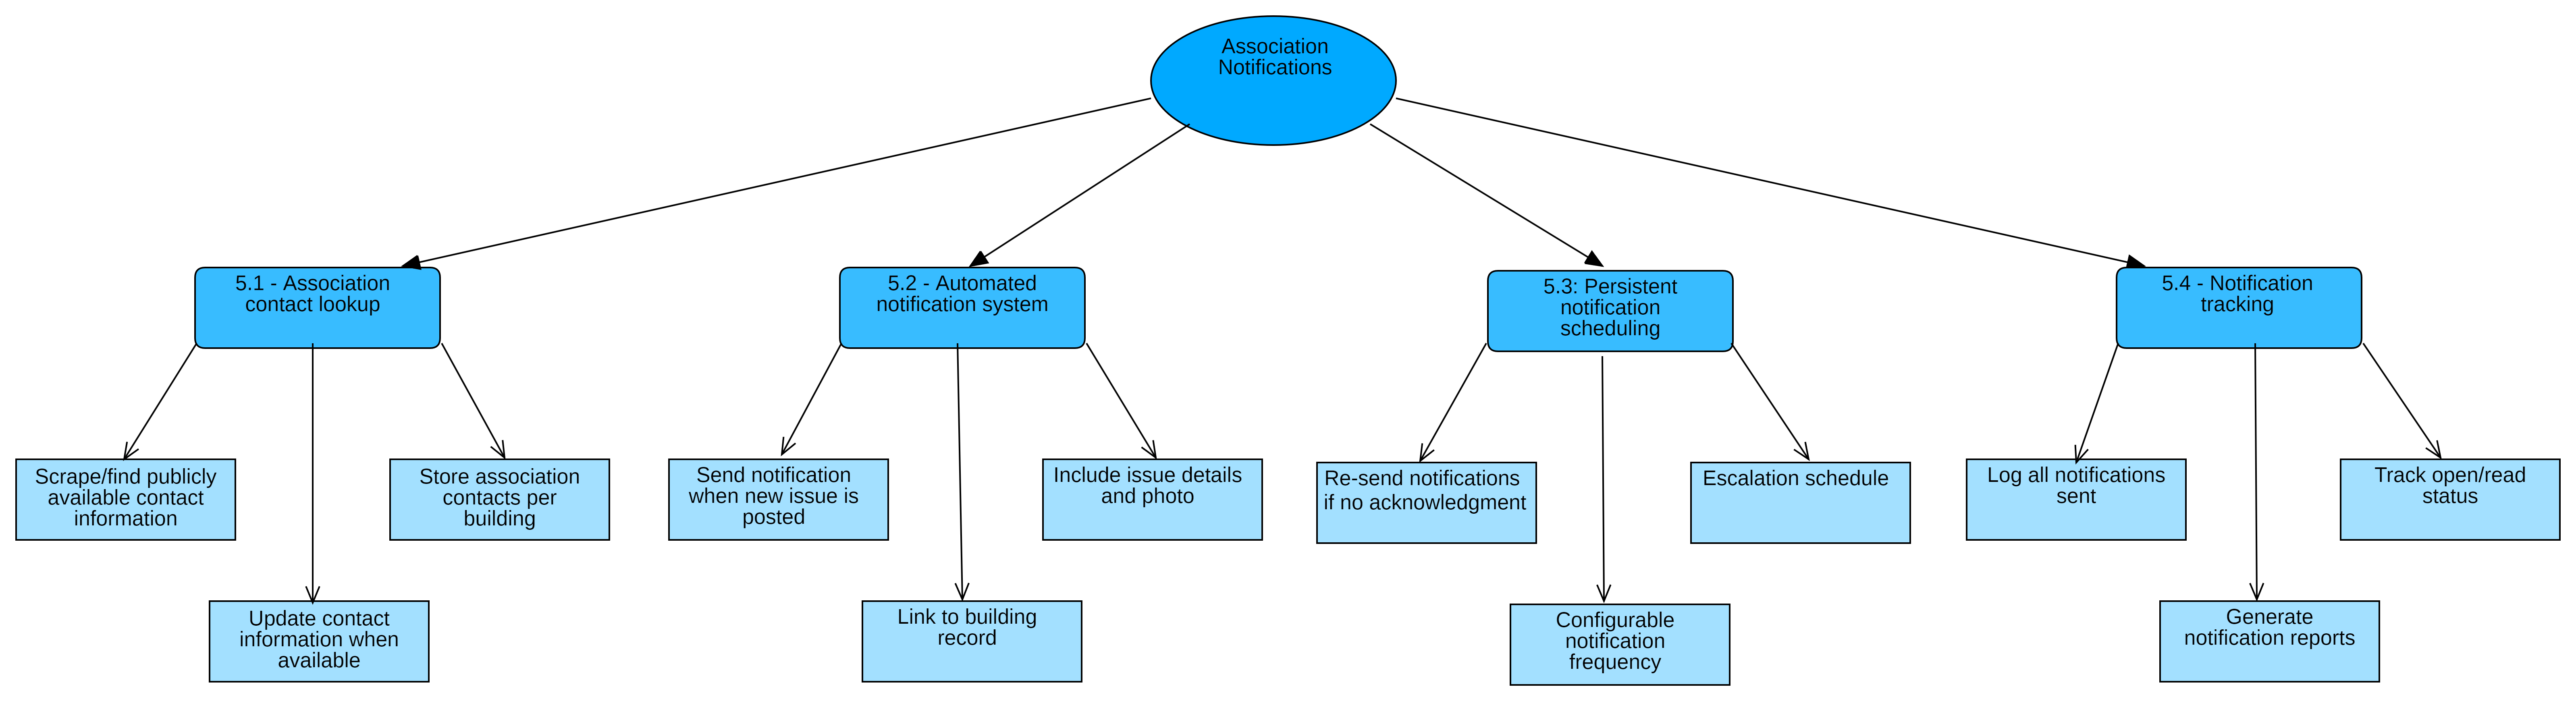
\includegraphics[height=0.2\textheight, keepaspectratio]{architecture/association management.png}
\caption{Association Management Interface}
\label{fig:association_management}
\end{figure}

Figure \ref{fig:association_management} above shows the Association Management interface. The current implementation sends email notifications via SendGrid when new issues are reported. Advanced features such as persistent scheduling, escalation workflows, and comprehensive dashboards are outside the scope of this project, as mentioned in Section 2.

\subsubsection{Public Visibility}

\begin{figure}[H]
\centering
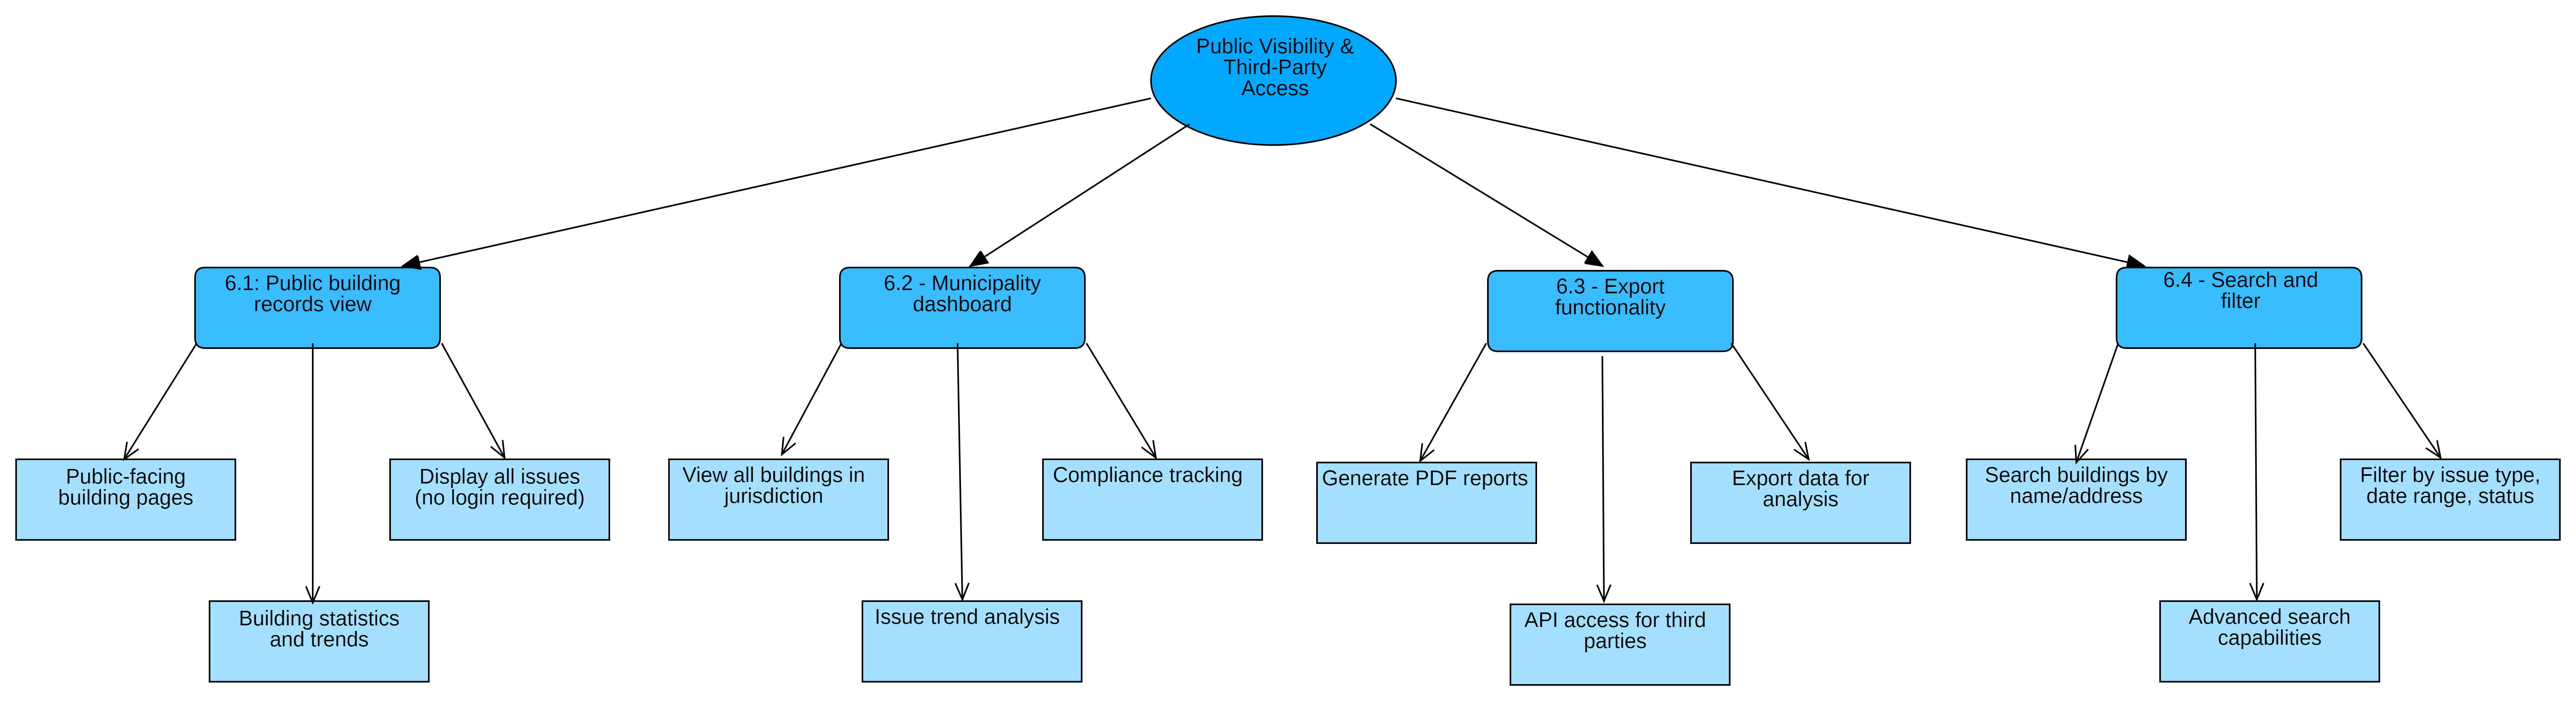
\includegraphics[height=0.2\textheight, keepaspectratio]{architecture/public_visibility.png}
\caption{Public Visibility Interface}
\label{fig:public_visibility}
\end{figure}

Figure \ref{fig:public_visibility} above shows the Public Visibility interface. Features such as public building records view, municipality dashboards, export functionality, and enhanced search capabilities are outside the scope of the current work but we will aim to add them in this iteration.

\subsection{Module Interfaces}

Module interfaces define the specific function calls and data structures used for communication between components. Detailed interface specifications will be defined during implementation based on the component relationships described above.

\subsection{User Interfaces (GUI)}

\subsubsection{Start Screen}

\begin{figure}[H]
\centering
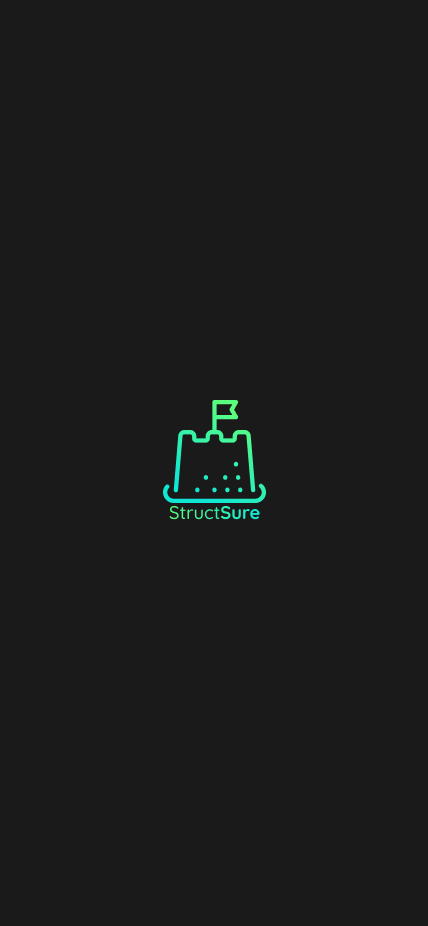
\includegraphics[height=0.25\textheight, keepaspectratio]{UI/start.png}
\caption{Start/Landing Screen}
\label{fig:start_screen}
\end{figure}

Figure \ref{fig:start_screen} above shows the start/landing screen of the mobile application. First time and returning users are presented with this screen, which serves as the entry point for authentication and system access.

\subsubsection{Homepage}

\begin{figure}[H]
\centering
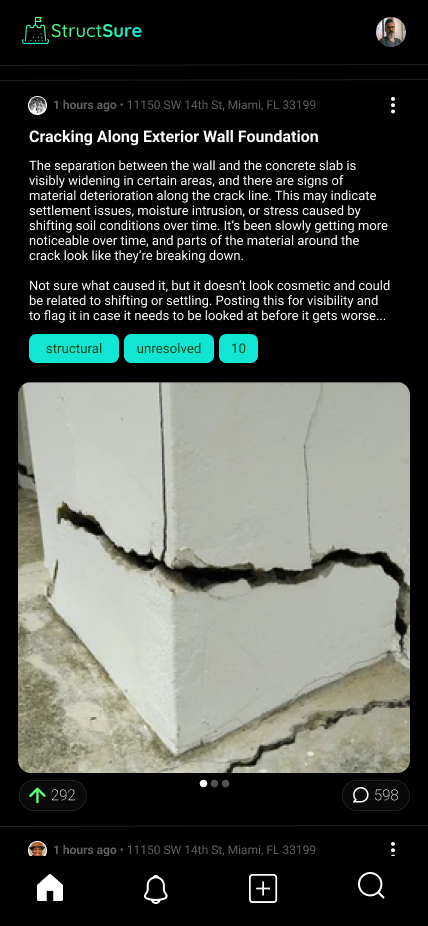
\includegraphics[height=0.25\textheight, keepaspectratio]{UI/homepage.png}
\qquad
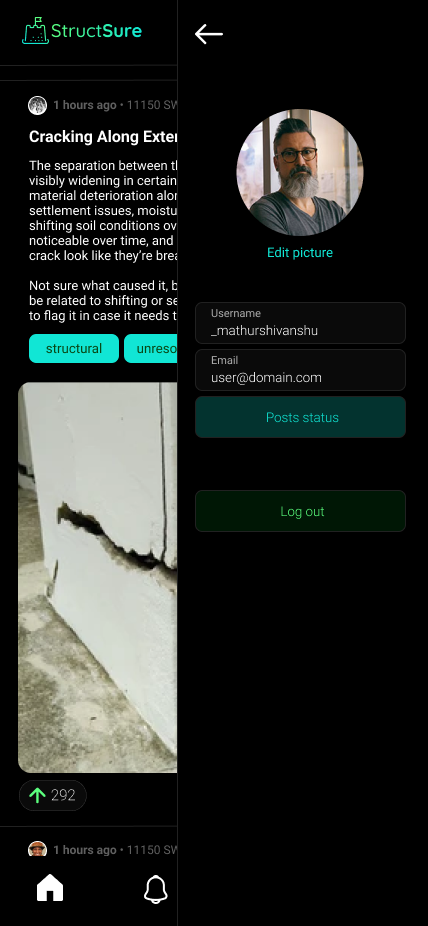
\includegraphics[height=0.25\textheight, keepaspectratio]{UI/homepage-profile.png}
\caption{Main Homepage and Homepage with Profile View}
\label{fig:homepage}
\end{figure}

Figure \ref{fig:homepage} above shows the main homepage and homepage with profile view. The main homepage provides navigation to the camera interface, user profile, notifications, and search functionality. The UI Controller presents this dashboard after successful authentication through the Session Manager. The homepage with profile view integrates the Resident Profile component, showing user identity and notification preferences alongside the main navigation.

\subsubsection{Photo Capture and Issue Creation}

\begin{figure}[H]
\centering
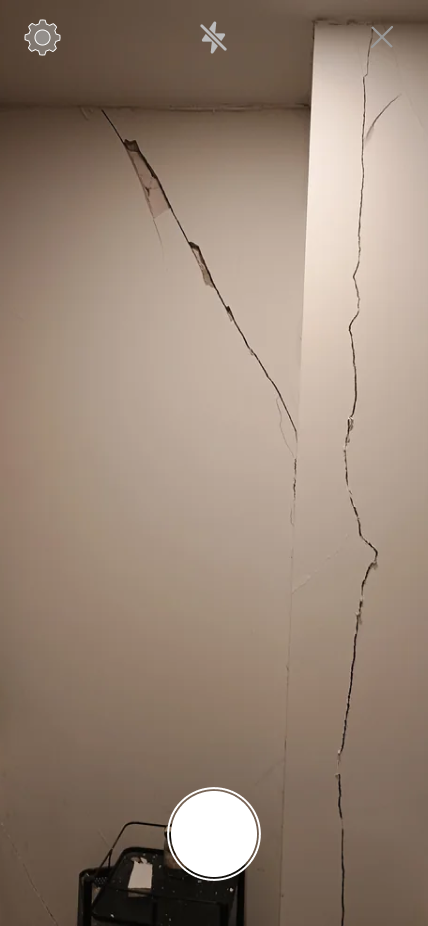
\includegraphics[height=0.25\textheight, keepaspectratio]{UI/camera.png}
\qquad
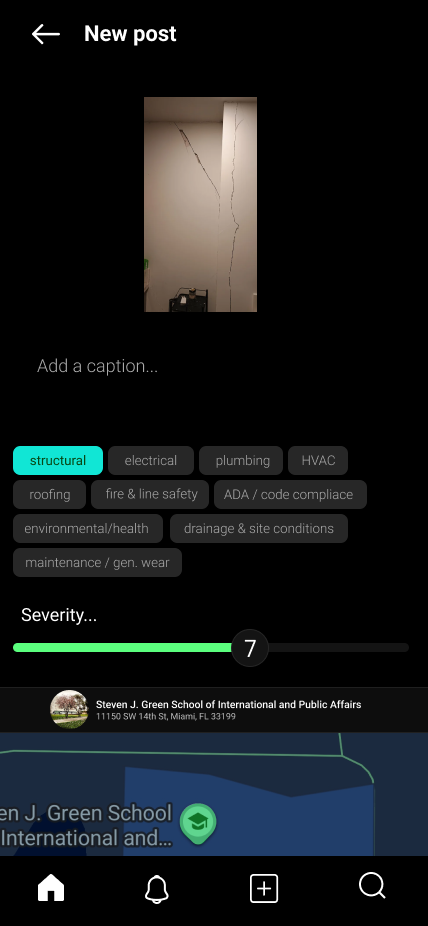
\includegraphics[height=0.25\textheight, keepaspectratio]{UI/post.png}
\caption{Camera Capture and Issue/Post Creation Screens}
\label{fig:photo_workflow}
\end{figure}

Figure \ref{fig:photo_workflow} above shows the camera capture interface and issue/post creation screen. Users can capture photos of infrastructure issues through the camera screen. Once a photo is captured, the system automatically captures GPS coordinates through the Geo/Map Controller. The photo capture is handled by the Expo SDK camera API as described in Section 2. After capturing a photo with location data, users can categorize the issue (e.g., structural, electrical, plumbing), provide an optional description, and select a severity rating on the post creation screen. This interface interacts with the Reporting API through the StructSure Core to create issue posts associated with buildings.

\subsubsection{User Profile Screen}

\begin{figure}[H]
\centering
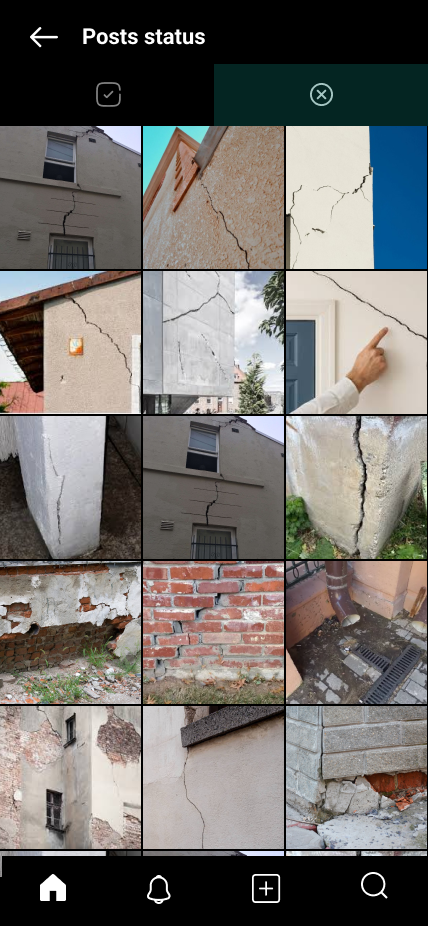
\includegraphics[height=0.25\textheight, keepaspectratio]{UI/user.png}
\caption{User Profile Screen}
\label{fig:user_profile}
\end{figure}

Figure \ref{fig:user_profile} above shows the user profile screen. This interface displays the Resident Profile information including identity, address, association information, and notification preferences. Profile data is managed through the StructSure Core and stored in the Database Manager.

\subsubsection{Notifications Screen}

\begin{figure}[H]
\centering
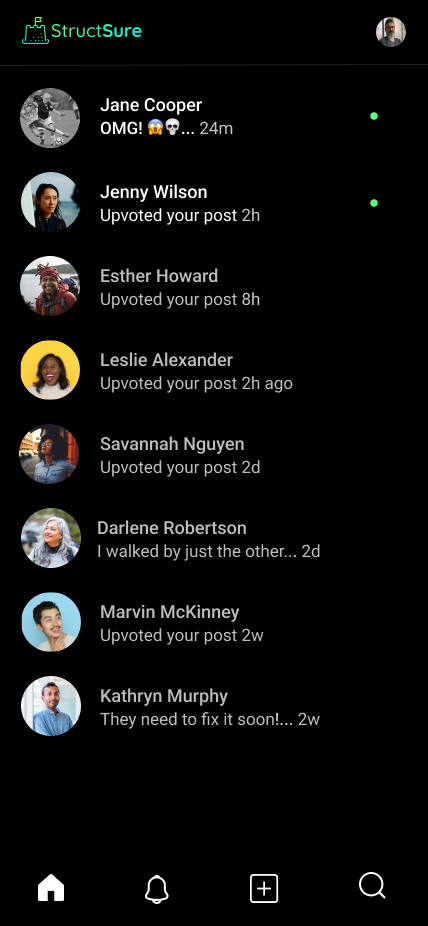
\includegraphics[height=0.25\textheight, keepaspectratio]{UI/notifications.png}
\caption{Notifications Screen}
\label{fig:notifications}
\end{figure}

Figure \ref{fig:notifications} above shows the notifications screen. This interface displays notifications related to reported issues, association responses, and system updates. The UI Controller retrieves notification data through the StructSure Core, which manages communication with the notification system.

\subsubsection{Search and Building History}

\begin{figure}[H]
\centering

\includegraphics[height=0.25\textheight, keepaspectratio]{UI/search-by-building.png}
\qquad
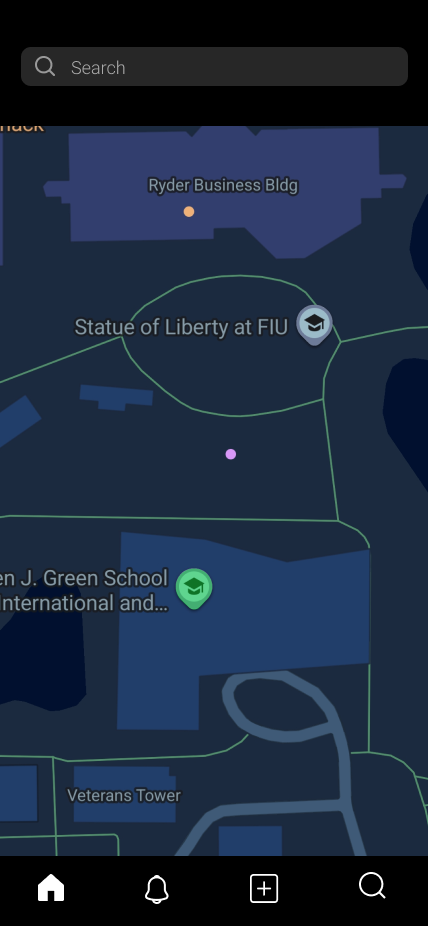
\includegraphics[height=0.25\textheight, keepaspectratio]{UI/search-by-map.png}
\caption{Search by Building and Search by Map Interfaces}
\label{fig:search_interfaces}
\end{figure}

Figure \ref{fig:search_interfaces} above shows the search interfaces. Users can search for buildings by name or address to view associated infrastructure issues, utilizing the Geo/Map Controller and Database Manager to retrieve building information. Users can also explore infrastructure issues by location on a map view, which integrates with the Google Places API through the Geo/Map Controller to display buildings and their associated issues geographically.

\begin{figure}[H]
\centering
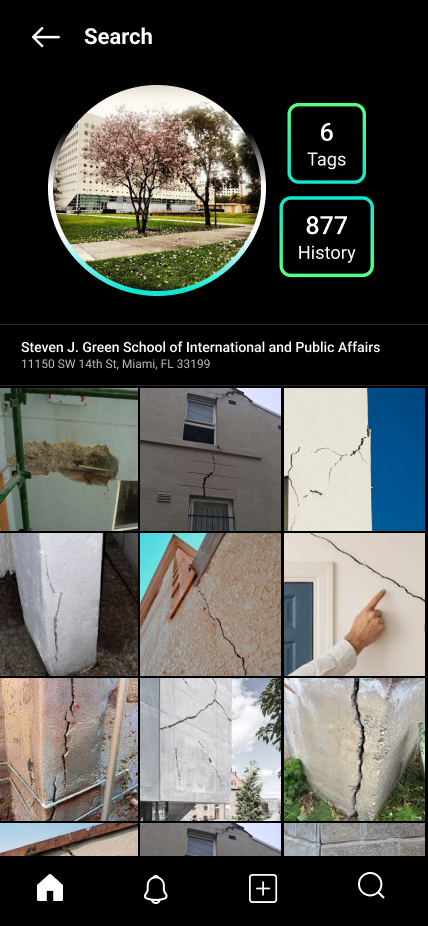
\includegraphics[height=0.25\textheight, keepaspectratio]{UI/search-building-history.png}
\qquad
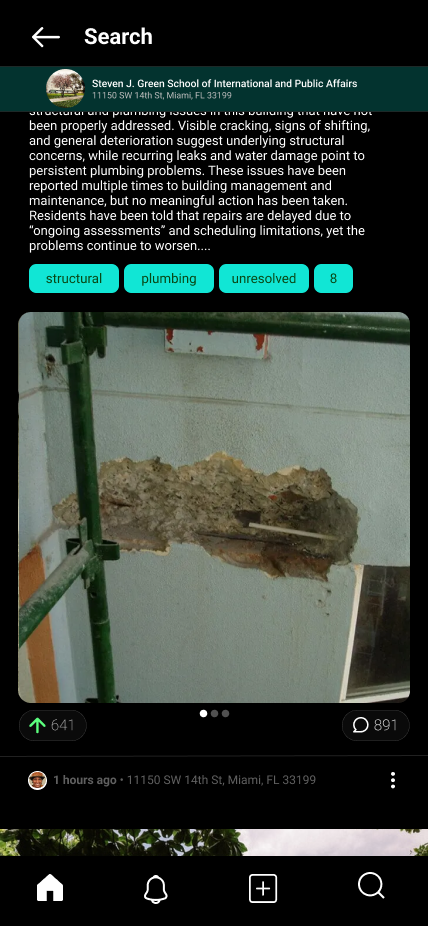
\includegraphics[height=0.25\textheight, keepaspectratio]{UI/search-review-building-history.png}
\caption{Building History Search and Review Interfaces}
\label{fig:building_history}
\end{figure}

Figure \ref{fig:building_history} above shows the building history search and review interfaces. The search results screen displays reported issues associated with specific buildings, with data provided by the Reporting API through the StructSure Core from the Database Manager. The review interface displays detailed building issue timelines, showing all reported issues for a selected building in chronological order. Each issue displays the photo, timestamp, category, and current status. Users can filter issues by date, category, or status. This functionality is implemented through the Reporting API and retrieves data from the Database Manager.

\newpage
\section{Detailed Design}

\textbf{Sequence Diagrams}

\begin{figure}[H]
    \centering
    \includegraphics[width=\textwidth, keepaspectratio]{system/sequence_diagram_SWE_2026.png}
    \caption{Sequence diagram showing the photo upload and building association workflow}
    \label{fig:sequence_diagram}
\end{figure}

\textbf{Pseudocode}

\begin{verbatim}
User opens camera interface
Request camera permission from device
If permission granted:
    Display camera preview
    Wait for user to tap capture button
    Capture photo from camera
    Request location permission from device
    If location permission granted:
        Get current GPS coordinates
        Extract EXIF metadata from photo
        Upload photo to Cloudinary with metadata
        Query Google Places API with GPS coordinates
        Display nearby building options to user
        Wait for user to select building
        Create issue post with photo URL, building ID, and metadata
        Store post in database
        Trigger notification to association
    Else:
        Display error: Location permission required
Else:
    Display error: Camera permission required
\end{verbatim}

\subsection{Data Detailed Design}

The system database extends Misskey's existing schema with the following main tables:

\begin{itemize}
    \item \textbf{Buildings Table}: Stores building information including name, address, GPS coordinates, Google Place ID, and association contact information.
    \item \textbf{Posts Table (Extended)}: Misskey's posts table extended with building association, issue category, severity rating, status, and location data.
    \item \textbf{Notifications Table}: Tracks email notifications sent to associations including recipient, timestamp, delivery status, and retry information.
\end{itemize}

\subsection{RTM}

\begin{tabular}{|p{3cm}|p{6cm}|p{4cm}|p{3cm}|}
\hline
\textbf{Requirement-ID} & \textbf{Requirement Description} & \textbf{Design Component} & \textbf{Test-Case \#} \\
\hline
FR-1 & User account creation with blog-style registration & Session Manager, User Profile & TBD \\
\hline
FR-2 & Camera-only photo capture (no gallery access) & Photo Capture Component & TBD \\
\hline
FR-3 & Real-time geo-location capture and tagging & Photo Capture Component, Building Management & TBD \\
\hline
FR-4 & Building identification via Google Places API & Building Management Component & TBD \\
\hline
FR-5 & Issue post creation linked to buildings & Photo Capture Component, Database Manager & TBD \\
\hline
FR-6 & Automated association notifications & Notification System & TBD \\
\hline
FR-7 & Public building records view & Public Access Component & TBD \\
\hline
FR-8 & Municipality dashboard & Public Access Component & TBD \\
\hline
FR-9 & Photo validation and abuse prevention & Photo Capture Component, Validation Module & TBD \\
\hline
\end{tabular}

\newpage
\section{Sprint Planning}

\setlist[enumerate]{topsep=0pt, partopsep=0pt, parsep=0pt, itemsep=2pt, leftmargin=1.5em}

\subsection{Role Focuses}

\vspace{0.3em}

\noindent
\begin{tabular}{|L{3cm}|L{4.5cm}|L{7.5cm}|}
\hline
\textbf{Team Member} & \textbf{Role} & \textbf{Responsibilities} \\
\hline
Grace Hechevarria & Frontend / UI Implementation Lead & Primary owner of React Native screens, camera flow, profile UI, notifications, search, and public pages \\
\hline
Nicole Fonseca & Frontend Integration \& Validation Lead & Handles permission flows, validation messages, session UI, error handling, and frontend protection \\
\hline
Logan Pritchard & Frontend Data Integration Lead & Connects UI to Google Places, Cloudinary, SendGrid responses, and manages data display \\
\hline
Andres Lopez & Backend Architecture \& API Lead & Owns Misskey backend, Python API wrapper, database schema, endpoints, issue logic, and notification triggers \\
\hline
\end{tabular}

\vspace{2em}

\subsection{Sprint Schedule, User Stories, and Acceptance Criteria}

\vspace{0.5em}

%%% SPRINT 1 %%%
\noindent{\textbf{\large Sprint 1 -- Account Creation \& Login}}

\vspace{0.5em}

\noindent
\begin{tabular}{|L{1.2cm}|L{1.8cm}|L{5.2cm}|L{6.3cm}|}
\hline
\textbf{Sprint} & \textbf{Dates} & \textbf{User Stories} & \textbf{Acceptance Criteria} \\
\hline
Sprint 1 & 02/08 -- 02/14 &
As a new user, I want to create an account with a username and optional email, so that I can use the system without strict verification. &
\begin{enumerate}
    \item Verify that a user can register with a username and password.
    \item Verify that email is optional.
    \item Verify that usernames are unique.
    \item Verify that successful registration logs the user in.
\end{enumerate} \\
\cline{3-4}
& &
As a user, I want to log in and log out, so that my account remains secure. &
\begin{enumerate}
    \item Verify that users can log in with valid credentials.
    \item Verify that logging out ends the session.
    \item Verify that protected routes require authentication.
\end{enumerate} \\
\hline
\end{tabular}

\vspace{0.5em}

\noindent
\begin{tabular}{|L{2.5cm}|L{12.5cm}|}
\hline
\textbf{Team Member} & \textbf{Task} \\
\hline
Grace & Login and registration screens \\
\hline
Nicole & Session validation messages and route protection UI \\
\hline
Logan & Display user profile data on UI after login \\
\hline
Andres & Build authentication API and connect to user model/database \\
\hline
\end{tabular}

\vspace{2em}

%%% SPRINT 2 %%%
\noindent{\textbf{\large Sprint 2 -- Camera-Only Photo Capture}}

\vspace{0.5em}

\noindent
\begin{tabular}{|L{1.2cm}|L{1.8cm}|L{5.2cm}|L{6.3cm}|}
\hline
\textbf{Sprint} & \textbf{Dates} & \textbf{User Stories} & \textbf{Acceptance Criteria} \\
\hline
Sprint 2 & 02/09 -- 02/15 &
As a user, I want to take photos using the in-app camera, so that only real-time images can be submitted. &
\begin{enumerate}
    \item Verify that camera permission is requested.
    \item Verify that no gallery or file upload option exists.
    \item Verify that photos come directly from the camera API.
\end{enumerate} \\
\hline
\end{tabular}

\vspace{0.5em}

\noindent
\begin{tabular}{|L{2.5cm}|L{12.5cm}|}
\hline
\textbf{Team Member} & \textbf{Task} \\
\hline
Grace & Expo Camera integration and capture screen \\
\hline
Nicole & Permission prompts and error messages \\
\hline
Logan & UI flow for camera preview and confirmation \\
\hline
Andres & Backend endpoint to receive image data \\
\hline
\end{tabular}

\vspace{2em}

%%% SPRINT 3 %%%
\noindent{\textbf{\large Sprint 3 -- Automatic Upload to Cloudinary}}

\vspace{0.5em}

\noindent
\begin{tabular}{|L{1.2cm}|L{1.8cm}|L{5.2cm}|L{6.3cm}|}
\hline
\textbf{Sprint} & \textbf{Dates} & \textbf{User Stories} & \textbf{Acceptance Criteria} \\
\hline
Sprint 3 & 02/16 -- 02/22 &
As a user, I want my photo to upload immediately after capture, so that it is securely stored with metadata. &
\begin{enumerate}
    \item Verify that upload starts automatically after capture.
    \item Verify that uploads include a server-side timestamp.
    \item Verify that users can see whether the upload succeeds or fails.
\end{enumerate} \\
\hline
\end{tabular}

\vspace{0.5em}

\noindent
\begin{tabular}{|L{2.5cm}|L{12.5cm}|}
\hline
\textbf{Team Member} & \textbf{Task} \\
\hline
Grace & Upload progress and success/failure display \\
\hline
Nicole & Frontend validation if upload fails \\
\hline
Logan & Connect UI to Cloudinary response data \\
\hline
Andres & Implement upload handling, timestamps, and metadata storage \\
\hline
\end{tabular}

\vspace{2em}

%%% SPRINT 4 %%%
\noindent{\textbf{\large Sprint 4 -- GPS Location Capture}}

\vspace{0.5em}

\noindent
\begin{tabular}{|L{1.2cm}|L{1.8cm}|L{5.2cm}|L{6.3cm}|}
\hline
\textbf{Sprint} & \textbf{Dates} & \textbf{User Stories} & \textbf{Acceptance Criteria} \\
\hline
Sprint 4 & 02/23 -- 03/01 &
As a user, I want my GPS location captured when I take a photo, so that issues show where it happened. &
\begin{enumerate}
    \item Verify that location permission is requested.
    \item Verify that submissions without GPS data are blocked.
    \item Verify that valid latitude and longitude values are stored.
\end{enumerate} \\
\hline
\end{tabular}

\vspace{0.5em}

\noindent
\begin{tabular}{|L{2.5cm}|L{12.5cm}|}
\hline
\textbf{Team Member} & \textbf{Task} \\
\hline
Grace & GPS capture integration into UI flow \\
\hline
Nicole & Permission prompts and error handling UI \\
\hline
Logan & Display coordinates/building suggestions on UI \\
\hline
Andres & Store GPS data and attach to issue metadata \\
\hline
\end{tabular}

\vspace{2em}

%%% SPRINT 5 %%%
\noindent{\textbf{\large Sprint 5 -- Building Identification with Google Places}}

\vspace{0.5em}

\noindent
\begin{tabular}{|L{1.2cm}|L{1.8cm}|L{5.2cm}|L{6.3cm}|}
\hline
\textbf{Sprint} & \textbf{Dates} & \textbf{User Stories} & \textbf{Acceptance Criteria} \\
\hline
Sprint 5 & 03/02 -- 03/08 &
As a user, I want to see nearby buildings suggested, so that I can accurately tag an issue. &
\begin{enumerate}
    \item Verify that nearby buildings are retrieved using GPS coordinates.
    \item Verify that results include building name and address.
\end{enumerate} \\
\cline{3-4}
& &
As a user, I want to select the correct building, so that the issue is linked accurately. &
\begin{enumerate}
    \item Verify that a building can be selected from the suggestion list.
    \item Verify that the selected building is stored with the issue.
\end{enumerate} \\
\hline
\end{tabular}

\vspace{0.5em}

\noindent
\begin{tabular}{|L{2.5cm}|L{12.5cm}|}
\hline
\textbf{Team Member} & \textbf{Task} \\
\hline
Grace & Building selection interface \\
\hline
Nicole & Validation if no building is selected \\
\hline
Logan & Display nearby buildings using API data \\
\hline
Andres & Process and store building ID with issue \\
\hline
\end{tabular}

\vspace{2em}

%%% SPRINT 6 %%%
\noindent{\textbf{\large Sprint 6 -- Issue Creation \& Building History}}

\vspace{0.5em}

\noindent
\begin{tabular}{|L{1.2cm}|L{1.8cm}|L{5.2cm}|L{6.3cm}|}
\hline
\textbf{Sprint} & \textbf{Dates} & \textbf{User Stories} & \textbf{Acceptance Criteria} \\
\hline
Sprint 6 & 03/09 -- 03/15 &
As a user, I want to create an issue with a photo and building, so that infrastructure problems are documented. &
\begin{enumerate}
    \item Verify that issue records store photo, building, timestamp, and user ID.
    \item Verify that the issue appears after submission.
\end{enumerate} \\
\cline{3-4}
& &
As a user, I want to view issues for a building in chronological order, so that I can view its history. &
\begin{enumerate}
    \item Verify that issues are ordered by date.
    \item Verify that resolved issues remain visible.
\end{enumerate} \\
\hline
\end{tabular}

\vspace{0.5em}

\noindent
\begin{tabular}{|L{2.5cm}|L{12.5cm}|}
\hline
\textbf{Team Member} & \textbf{Task} \\
\hline
Grace & Issue creation form and history display UI \\
\hline
Nicole & UI validation for required fields \\
\hline
Logan & Populate building issue history from API data \\
\hline
Andres & Build issue creation endpoint and database schema \\
\hline
\end{tabular}

\vspace{2em}

%%% SPRINT 7 %%%
\noindent{\textbf{\large Sprint 7 -- Association Email Notifications}}

\vspace{0.5em}

\noindent
\begin{tabular}{|L{1.2cm}|L{1.8cm}|L{5.2cm}|L{6.3cm}|}
\hline
\textbf{Sprint} & \textbf{Dates} & \textbf{User Stories} & \textbf{Acceptance Criteria} \\
\hline
Sprint 7 & 03/16 -- 03/22 &
As the system, I want to notify associations when an issue is posted, so that they're aware and can take action. &
\begin{enumerate}
    \item Verify that emails are sent on issue creation.
    \item Verify that emails include issue details and links.
    \item Verify that failed notifications are logged.
\end{enumerate} \\
\hline
\end{tabular}

\vspace{0.5em}

\noindent
\begin{tabular}{|L{2.5cm}|L{12.5cm}|}
\hline
\textbf{Team Member} & \textbf{Task} \\
\hline
Grace & Notification status UI \\
\hline
Nicole & Error/status messages for notifications \\
\hline
Logan & Display association contact/notification results \\
\hline
Andres & Trigger SendGrid emails and log results \\
\hline
\end{tabular}

\vspace{2em}

%%% SPRINT 8 %%%
\noindent{\textbf{\large Sprint 8 -- Abuse Prevention \& Validation}}

\vspace{0.5em}

\noindent
\begin{tabular}{|L{1.2cm}|L{1.8cm}|L{5.2cm}|L{6.3cm}|}
\hline
\textbf{Sprint} & \textbf{Dates} & \textbf{User Stories} & \textbf{Acceptance Criteria} \\
\hline
Sprint 8 & 03/23 -- 03/29 &
As the system, I want to limit submissions per user, so that spam and abuse are reduced. &
\begin{enumerate}
    \item Verify that daily submission limits are enforced.
    \item Verify that users receive an error when limits are exceeded.
\end{enumerate} \\
\cline{3-4}
& &
As the system, I want to detect duplicate photo uploads, so that repeated spam is prevented. &
\begin{enumerate}
    \item Verify that duplicate images are detected using file hashing.
    \item Verify that duplicate submissions are blocked or flagged.
\end{enumerate} \\
\hline
\end{tabular}

\vspace{0.5em}

\noindent
\begin{tabular}{|L{2.5cm}|L{12.5cm}|}
\hline
\textbf{Team Member} & \textbf{Task} \\
\hline
Grace & User feedback when limits are reached \\
\hline
Nicole & UI for duplicate/limit errors \\
\hline
Logan & Show validation results on screen \\
\hline
Andres & Implement submission limits and hashing logic \\
\hline
\end{tabular}

\vspace{2em}

%%% SPRINT 9 %%%
\noindent{\textbf{\large Sprint 9 -- Public Building View \& Search}}

\vspace{0.5em}

\noindent
\begin{tabular}{|L{1.2cm}|L{1.8cm}|L{5.2cm}|L{6.3cm}|}
\hline
\textbf{Sprint} & \textbf{Dates} & \textbf{User Stories} & \textbf{Acceptance Criteria} \\
\hline
Sprint 9 & 03/30 -- 04/05 &
As a member of the public, I want to view building issue records without logging in, so that transparency is maintained. &
\begin{enumerate}
    \item Verify that public building pages are accessible without authentication.
    \item Verify that no private user data is exposed.
\end{enumerate} \\
\cline{3-4}
& &
As a user, I want to search and filter building issues, so that I can find relevant records efficiently. &
\begin{enumerate}
    \item Verify that buildings can be searched by name or address.
    \item Verify that issues can be filtered by date or status.
\end{enumerate} \\
\hline
\end{tabular}

\vspace{0.5em}

\noindent
\begin{tabular}{|L{2.5cm}|L{12.5cm}|}
\hline
\textbf{Team Member} & \textbf{Task} \\
\hline
Grace & Public building view screens \\
\hline
Nicole & Ensure UI hides private user data \\
\hline
Logan & Search UI and results display \\
\hline
Andres & Build public endpoints and secure data filtering \\
\hline
\end{tabular}

\vspace{2em}

\begin{figure}[H]
\centering
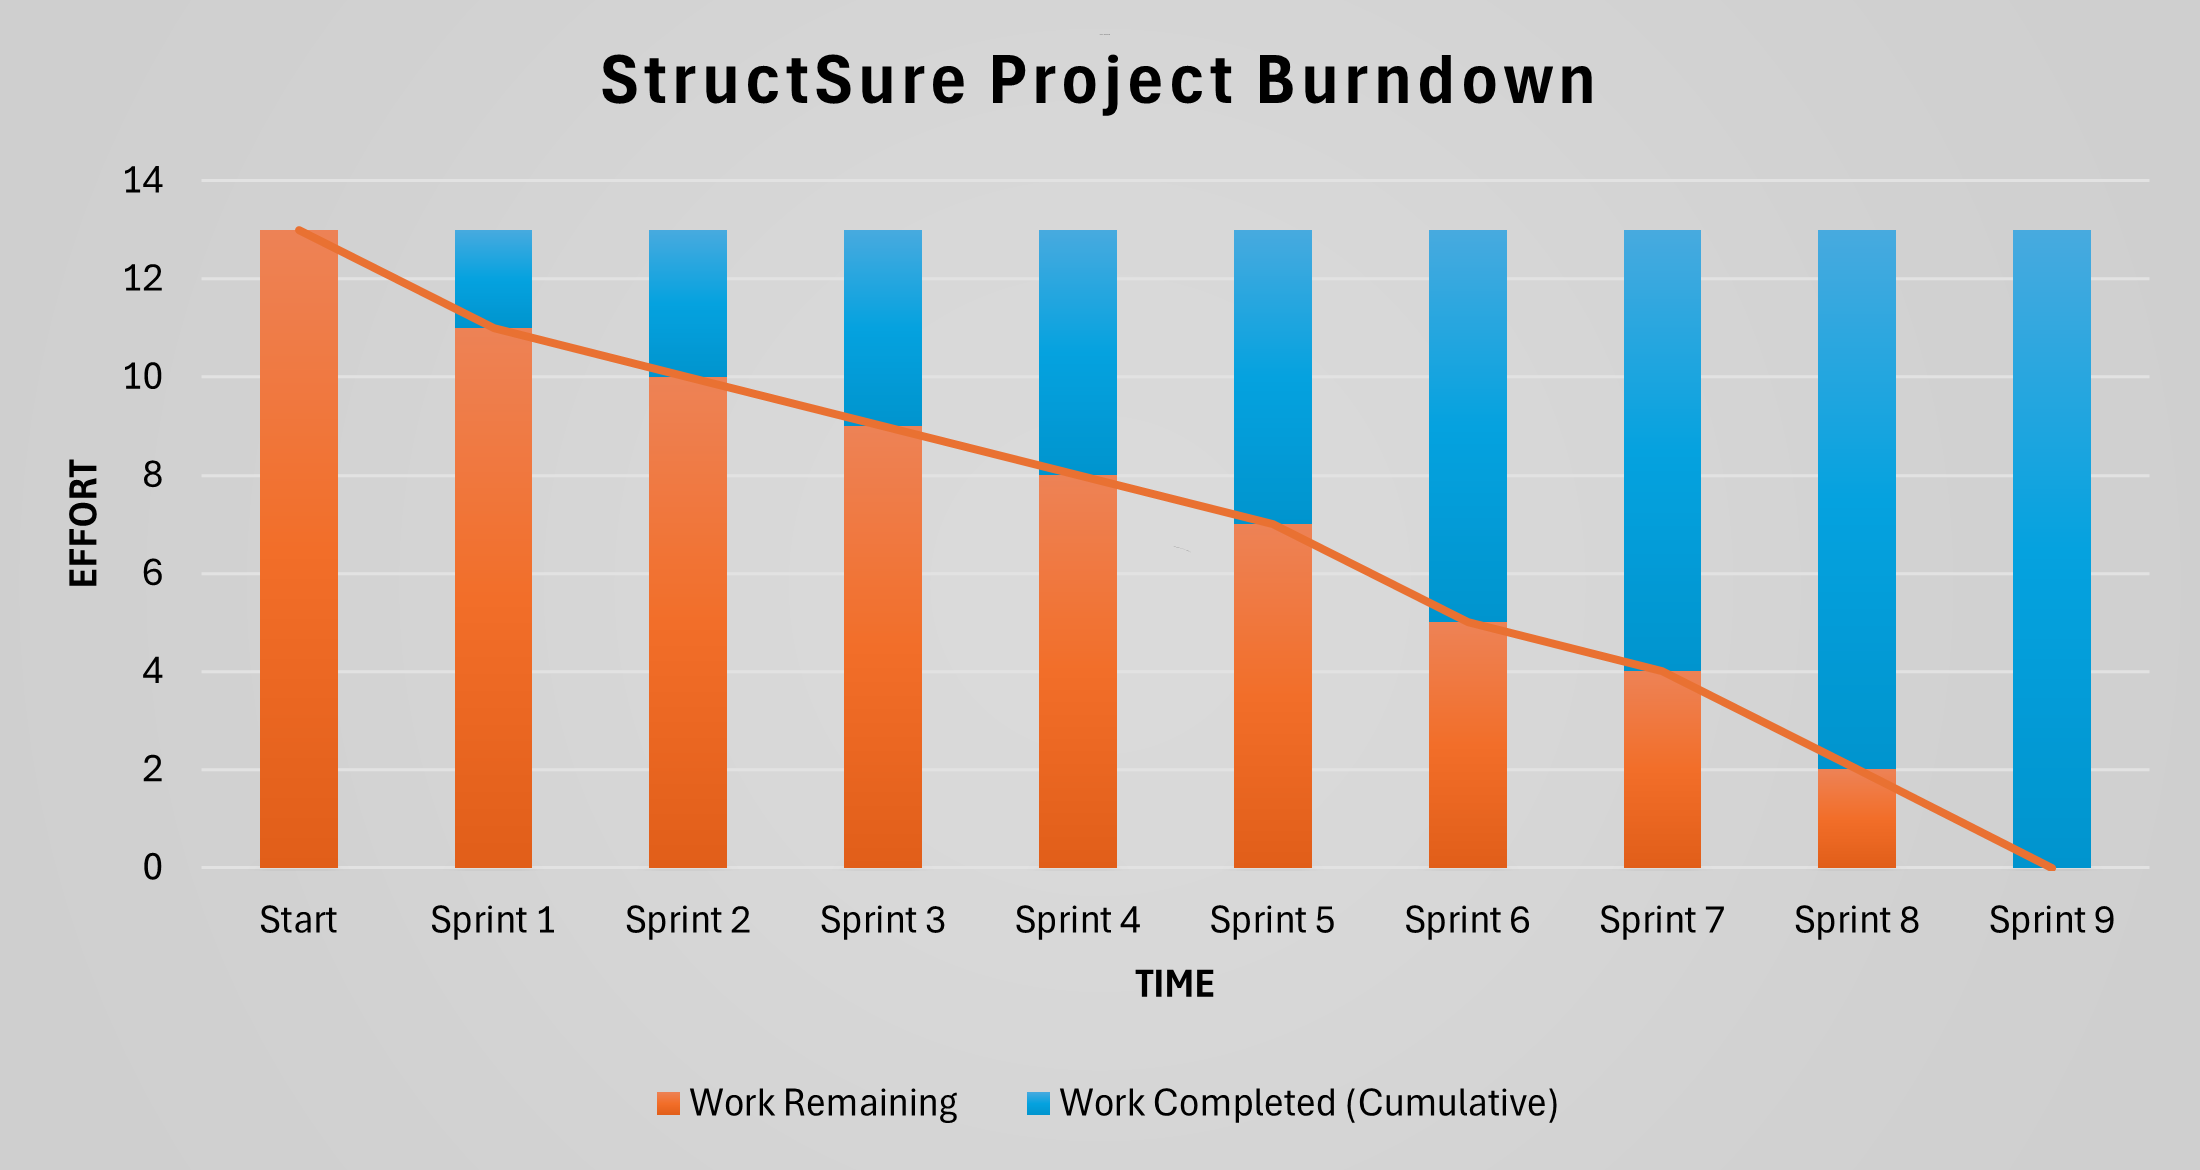
\includegraphics[width=\textwidth, keepaspectratio]{sprint/StructSure_Project_Burndown_Chart.png}
\caption{StructSure project burndown chart. A burndown chart shows remaining work over time so the team can track progress and predict completion.}
\label{fig:burndown}
\end{figure}

\end{document}
